%=================================================================
% MIT LICENSE
%=================================================================
% Copyright (c) 2022 Techneatium
%
% Permission is hereby granted, free of charge, to any person obtaining a copy
% of this software and associated documentation files (the "Software"), to deal
% in the Software without restriction, including without limitation the rights
% to use, copy, modify, merge, publish, distribute, sublicense, and/or sell
% copies of the Software, and to permit persons to whom the Software is
% furnished to do so, subject to the following conditions:
%
% The above copyright notice and this permission notice shall be included in all
% copies or substantial portions of the Software.
%
% THE SOFTWARE IS PROVIDED "AS IS", WITHOUT WARRANTY OF ANY KIND, EXPRESS OR
% IMPLIED, INCLUDING BUT NOT LIMITED TO THE WARRANTIES OF MERCHANTABILITY,
% FITNESS FOR A PARTICULAR PURPOSE AND NONINFRINGEMENT. IN NO EVENT SHALL THE
% AUTHORS OR COPYRIGHT HOLDERS BE LIABLE FOR ANY CLAIM, DAMAGES OR OTHER
% LIABILITY, WHETHER IN AN ACTION OF CONTRACT, TORT OR OTHERWISE, ARISING FROM,
% OUT OF OR IN CONNECTION WITH THE SOFTWARE OR THE USE OR OTHER DEALINGS IN THE
% SOFTWARE.
%=================================================================

%-----------------------------------------------------------------
% BEGIN DOCUMENT
%-----------------------------------------------------------------
\documentclass[fontHelvetica, widesubsec]{TechCheck}
\title{F18_Cheatsheet}
\author{Techneatium}

\setaircraftlong{F/A-18C AIRCRAFT} % sets long label for title page
\setaircraftshort{F/A-18C} % sets short label for header
\settabnumber{8} % sets number of tabs for document

\begin{document}
	%-----------------------------------------------------------------
% TITLE PAGE
%-----------------------------------------------------------------
	% deactivate header and footer
	\pagestyle{empty}
	\newlength{\centeroffset}
	\setlength\centeroffset{(\chevin-\outmar-0.5cm)/2}
	\begin{tikzpicture}[overlay, remember picture]
	\node[
	]() at ([xshift=\centeroffset,yshift=8.5cm]current page.center) {
		\Huge \titlefont\textbf{Pocket Checklist}
	};
	\node[
	]() at ([xshift=\centeroffset,yshift=7cm]current page.center) {
		\resizebox{10cm}{!}{\titlefont\textbf{\colorbox{color1}{\textcolor{white}{\aircraftlong}}}}
	};
	\node[
	]() at ([xshift=\centeroffset,yshift=5.5cm]current page.center) {
		\Large \titlefont\textbf{\colorbox{color1}{\textcolor{white}{REV: \today}}} \blue{}
	};
	\node[
	]() at ([xshift=\centeroffset,yshift=-1cm]current page.center) {
		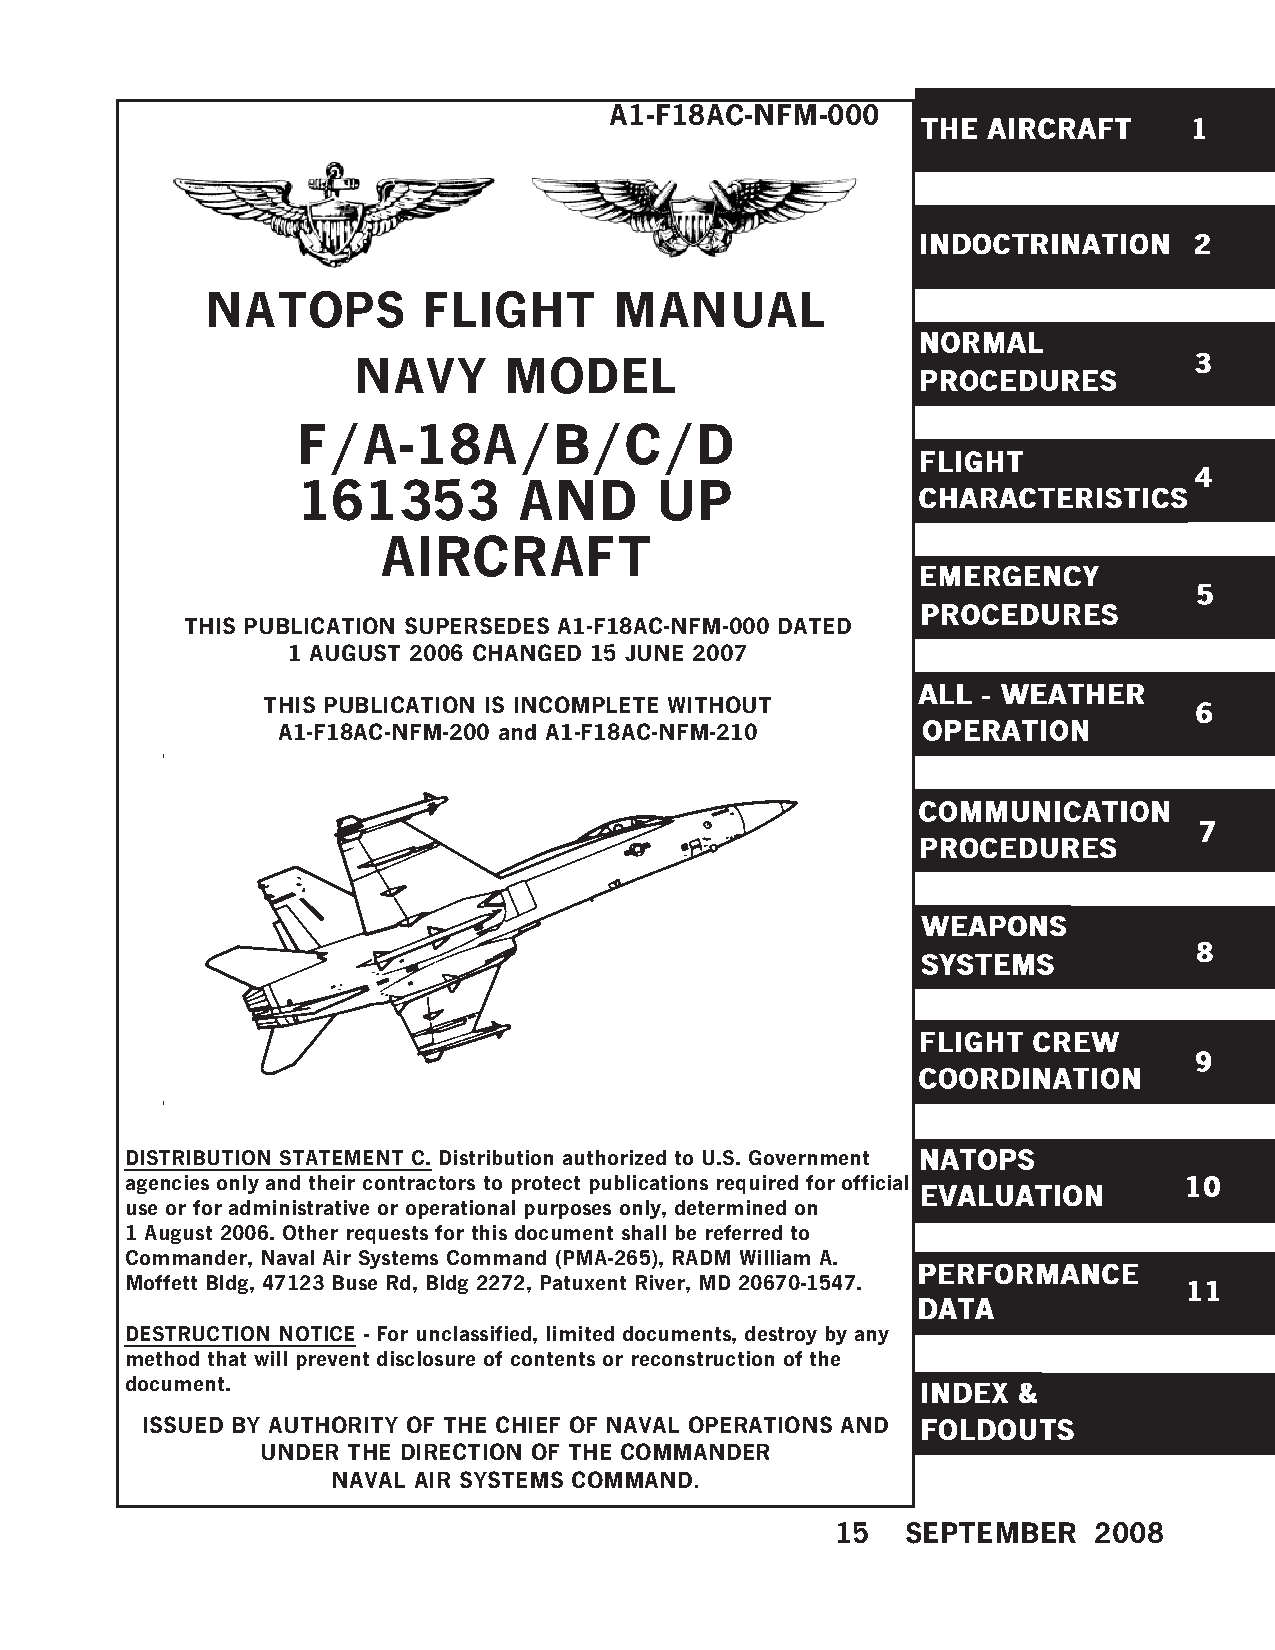
\includegraphics[
			width=0.8\linewidth,
			page = {1},
			trim = {3.0cm, 9.5cm, 8.0cm, 13cm},
			clip
		]{natops_F18C.pdf}
	};
	% Black area for white chevrons
	\fill[color1]
		([xshift=\outmar, yshift=0.2cm]current page text area.north east) --
		([xshift=\outmar, yshift=-\botmar]current page text area.south east) --
		([xshift=\chevin-0.5cm, yshift=-\botmar]current page text area.south east) --
		([xshift=\chevin-0.5cm, yshift=0.2cm]current page text area.north east) --
		cycle;
	\end{tikzpicture}
	% label for hyperrefs back to frontpage
	\label{frontpage}
	% make chevrons
	% use tabular for multi line node
	\thumbfront{Procedures}{0}
	\thumbfront{\begin{tabular}{c} Systems \end{tabular}}{1}
	\thumbfront{\begin{tabular}{c} APG-73 \\ Radar \end{tabular}}{2}
	\thumbfront{\begin{tabular}{c} TGP \\ JHMCS \end{tabular}}{3}
	\thumbfront{\begin{tabular}{c} A/G \\ Weapons \end{tabular}}{4}
	\thumbfront{\begin{tabular}{c} A/A \\ Weapons \end{tabular}}{5}
	\thumbwide

	\clearpage
	\null\vspace{0cm}

	\begin{tcolorbox}[
		enhanced, colback=white, colframe=color1, colbacktitle=white, coltitle=color1, sharp corners, attach boxed title to top center={yshift=2mm},
		boxed title style={
			sharp corners,
			drop shadow=color1!100
		}, title=\LARGE\textbf{DISCLAIMER}
	]
		\textbf{This document represents a personal project and is intended for entertainment purposes only. Do not use for training purposes or in real life scenarios.}
	\end{tcolorbox}

	\cleardoublepage

	\thumbnar
	\dominitoc
	\tableofcontents
	\cleardoublepage

	% restart page counter
	\setcounter{page}{1}
	% reactivate header and footer
	\pagestyle{body}

	\chapter{PROCEDURES}
	\thumbtab{Procedures}{0}
	\minitoc
	\cleardoublepage

	\section{START-UP}
	\subsection{PRE-START}
	\begin{center}
		\begin{longtable}{l p{3cm} | p{8cm}}
			\toprule
			1. & \blue{Ejection Seat test} & \textbf{DOWN \& ARMED} \\
			\midrule
			2. & \blue{Harness Lever} & \textbf{FWD} \\
			\midrule
			3. & \blue{Parking Brake} & \textbf{ENGAGED} \\
			\midrule
			4. & \blue{Master Arm} & \textbf{SAFE} \\
			\bottomrule
		\end{longtable}
	\end{center}

	\subsection{ENGINE START}
	\begin{center}
		\begin{longtable}{l p{3cm} | p{8cm}}
			\toprule
			1. & \blue{Battery} & \textbf{ON} \\
			\midrule
			2. & \blue{Hyd. Brake} & > 3000psi \\
			\midrule
			3. & \blue{Fire Test} &
			\begin{minipage}[t]{\linewidth}
				\vspace{-7pt}
				\begin{enumerate}
					\item \textbf{FIRE TEST} \dotfill \textbf{TEST A}
					\item \textbf{BATT} \dotfill cycle \textbf{OFF} then \textbf{ON}
					\item \textbf{FIRE TEST} \dotfill \textbf{TEST B}
				\end{enumerate}
			\end{minipage} \\
			\midrule
			4. & \blue{APU Start} &
			\begin{minipage}[t]{\linewidth}
				\vspace{-7pt}
				\begin{enumerate}
					\item \textbf{APU Caution Light} \dotfill verify OFF
					\item \textbf{APU Switch} \dotfill \textbf{ON} \\
					\item \textbf{READY Light} \dotfill illuminated (30s)
				\end{enumerate}
			\end{minipage} \\
			\midrule
			5. & \blue{Right Engine Start} &
			\begin{minipage}[t]{\linewidth}
				\vspace{-7pt}
				\begin{enumerate}
					\item \textbf{ENG CRANK} \dotfill \textbf{R}
					\item \textbf{R Eng RPM} \dotfill 15-25\%
					\item \textbf{R Throttle} \dotfill \textbf{IDLE}
				\end{enumerate}
			\end{minipage} \\
			\midrule
			6. & \blue{Stabilized Parameters} &
			\begin{minipage}[t]{\linewidth}
				\vspace{-7pt}
				\begin{itemize}
					\item \textbf{IFEI} \dotfill Check
					\begin{itemize}
						\item \textbf{RPM} -- 60-65\%
						\item \textbf{EGT} -- < 750C until stable
					\end{itemize}
					\item \textbf{Cautions} \dotfill none for \textbf{ENG 2}
					\item \textbf{GPWS Voice Alerts} \dotfill Check
				\end{itemize}
			\end{minipage} \\
			\midrule
			7. & \blue{Master Caution} & \textbf{RESET} \\
			\midrule
			8. & \blue{Displays} &
			\begin{minipage}[t]{\linewidth}
				\vspace{-7pt}
				\begin{enumerate}
					\item \textbf{Left DDI} \dotfill \textbf{ON}
					\item \textbf{Right DDI} \dotfill \textbf{ON}
					\item \textbf{AMPCD} \dotfill \textbf{ON}
				\end{enumerate}
			\end{minipage} \\
			\midrule
			9. & \blue{UFC} &
			\begin{minipage}[t]{\linewidth}
				\vspace{-7pt}
				\begin{enumerate}
					\item \textbf{HUD} \dotfill \textbf{ON}
					\item \textbf{ALT Switch} \dotfill \textbf{RDR}
					\item \textbf{ATT Switch} \dotfill \textbf{AUTO}
				\end{enumerate}
			\end{minipage} \\
			\midrule
			10. & \blue{BLEED AIR Knob} & Cycle thru \textbf{OFF} to \textbf{NORM} \break (shutoff valves closed during fire test) \\
			\midrule
			11. & \blue{Left Engine Start} &
			\begin{minipage}[t]{\linewidth}
				\vspace{-7pt}
				\begin{enumerate}
					\item \textbf{ENG CRANK} \dotfill \textbf{L}
					\item \textbf{L Eng RPM} \dotfill 15-25\%
					\item \textbf{L Throttle} \dotfill \textbf{IDLE}
				\end{enumerate}
			\end{minipage} \\
			\midrule
			12. & \blue{Stabilized Parameters} &
			\begin{minipage}[t]{\linewidth}
				\vspace{-7pt}
				\begin{itemize}
					\item \textbf{IFEI} \dotfill Check
					\begin{itemize}
						\item \textbf{RPM} -- 60-65\%
						\item \textbf{EGT} -- < 750C until stable
					\end{itemize}
					\item \textbf{Cautions} \dotfill none for \textbf{ENG 1}
					\item \textbf{L GEN Caution} \dotfill Extinguished
				\end{itemize}
			\end{minipage} \\
			\bottomrule
		\end{longtable}
	\end{center}

	\subsection{POST-START}
	\begin{center}
		\begin{longtable}{l p{3cm} | p{8cm}}
			\toprule
			1. & \blue{Canopy} & \textbf{CLOSED} \\
			\midrule
			2. & \blue{Start INS Align} &
			\begin{minipage}[t]{\linewidth}
				\vspace{-7pt}
				\begin{enumerate}
					\item \textbf{INS Selector} \dotfill \textbf{GND} or \textbf{CV} (as required)
					\item \textbf{HSI} \dotfill select \textbf{STD HDG} (if available) \\ \hfill \emph{(significantly reduces align time to approx. 90s)}
				\end{enumerate}
			\end{minipage} \\
			\midrule
			3. & \blue{RADAR} & \textbf{OPR} \\
			\midrule
			4. & \blue{FCS Reset} &
			\begin{minipage}[t]{\linewidth}
				\vspace{-7pt}
				\begin{enumerate}
					\item \textbf{WING FOLD} \dotfill \textbf{SPREAD} \\
					\hfill \textbf{ONLY IF ON GROUND}
					\item \textbf{Left DDI} \dotfill \textbf{FCS} page
					\item \textbf{MASTER CAUTION} \dotfill \textbf{PRESS} twice \\ \hfill (restacks cautions)
					\item \textbf{FCS RESET} \dotfill \textbf{PRESS}
				\end{enumerate}
			\end{minipage} \\
			\midrule
			5. & \blue{Lights Test} & \textbf{Check} \\
			\midrule
			6. & \blue{Hook Bypass} & \textbf{As Required} \\
			\midrule
			7. & \blue{Flaps} & \textbf{HALF} \\
			\midrule
			8. & \blue{FCS BIT} &
			\begin{minipage}[t]{\linewidth}
				\vspace{-7pt}
				\begin{enumerate}
					\item \textbf{BIT Failures} \dotfill press FCS-MC
					\item \textbf{MC1 \& MC2} \dotfill GO
					\item \textbf{FCSA \& FCSB} \dotfill PBIT GO
					\item \textbf{FCS BIT Switch} \dotfill press \& hold
					\item \textbf{FCS-MC} \dotfill press FCS OSB
					\item \textbf{FCSA \& FCSB} \dotfill GO
				\end{enumerate}
			\end{minipage} \\
			\midrule
			9. & \blue{ANTI SKID} & \textbf{OFF} if CV, else \textbf{ON} \\
			\midrule
			10. & \blue{Trim} & \textbf{PRESS T/O Trim} \\
			\midrule
			11. & \blue{PITOT} & \textbf{AUTO} \\
			\midrule
			12. & \blue{Displays} &
			\begin{minipage}[t]{\linewidth}
				\vspace{-7pt}
				\begin{enumerate}
					\item \textbf{Left DDI} \dotfill \textbf{HUD Repeater}
					\item \textbf{Right DDI} \dotfill \textbf{FCS Page}
				\end{enumerate}
			\end{minipage} \\
			\midrule
			13. & \blue{RADALT Warning} &
			\begin{minipage}[t]{\linewidth}
				\vspace{-7pt}
				\begin{itemize}
					\item \textbf{GND}\dotfill 200 ft
					\item \textbf{CV}\dotfill 80 ft
				\end{itemize}
			\end{minipage} \\
			\midrule
			14. & \blue{Standby Attitude Indicator} & \textbf{UNCAGED} \\
			\midrule
			15. & \blue{Bingo Fuel} & \textbf{As desired} (8000lbs) \\
			\midrule
			16. & \blue{Altimeter} & \textbf{Set} \\
			\midrule
			17. & \blue{Mission Data} & \textbf{ENTER} \\
			\midrule
			18. & \blue{Weapons/Sensors} & \textbf{As Required} \\
			\midrule
			19. & \blue{STORES Page} & \textbf{Verify proper inventory installed} \\
			\midrule
			20. & \blue{HMD Alignment} &
			\begin{minipage}[t]{\linewidth}
				\vspace{-7pt}
				\begin{enumerate}
					\item \textbf{SUPT/HMD/ALIGN Page} \dotfill \textbf{SELECT}
					\item Superimpose \textbf{HMD} alignment cross on \textbf{HUD/BRU} alignment cross
					\item \textbf{CAGE/UNCAGE} \dotfill \textbf{PRESS \& HOLD} \\
					\hfill until \textbf{ALIGN OK}
				\end{enumerate}
				\textbf{Fine Align}
				\begin{enumerate}
					\item With \textbf{FA DXDY} displayed, use \textbf{TDC} to align azimuth and elevation \textbf{HMD} alignment crosses with \textbf{HUD/BRU} alignment cross
					\item \textbf{CAGE/UNCAGE} \dotfill \textbf{PRESS \& RELEASE}
					\item With \textbf{FA DROLL} displayed, use \textbf{TDC} to align roll axis \textbf{HMD} alignment crosses with \textbf{HUD/BRU} alignment cross
					\item \textbf{CAGE/UNCAGE} \dotfill \textbf{PRESS \& RELEASE}
				\end{enumerate}
			\end{minipage} \\
			\midrule
			21. & \blue{OBOGS} & \textbf{ON} \\
			\midrule
			22. & \blue{Complete INS Align} & \textbf{INS Selector} to \textbf{NAV} or \textbf{IFA} (if available) \\
			\midrule
			23. & \blue{Defensive Systems} &
			\begin{minipage}[t]{\linewidth}
				\vspace{-7pt}
				\begin{enumerate}
					\item \textbf{ALR-67 RWR} \dotfill \textbf{ON}
					\item \textbf{ECM Selector} \dotfill \textbf{STBY}
					\item \textbf{Dispenser} \dotfill \textbf{ON} (middle)
				\end{enumerate}
			\end{minipage} \\
			\midrule
			24. & \blue{Lights} &
			\begin{minipage}[t]{\linewidth}
				\vspace{-7pt}
				\begin{enumerate}
					\item \textbf{Strobe} \dotfill \textbf{ON}
					\item \textbf{POS Lights} \dotfill \textbf{BRT}
					\item \textbf{LDG/TAXI Lights} \dotfill \textbf{ON}
				\end{enumerate}
			\end{minipage} \\
			\midrule
			25. & \blue{Network} &
			\begin{minipage}[t]{\linewidth}
				\vspace{-7pt}
				\begin{enumerate}
					\item \textbf{IFF} \dotfill \textbf{ON}
					\item \textbf{D/L} \dotfill \textbf{ON}, set desired frequency
				\end{enumerate}
			\end{minipage} \\
			\midrule
			26. & \blue{Parking Brake} & \textbf{DISENGAGE} \\
			\midrule
			27. & \blue{Chocks} & \textbf{REMOVED} \\
			\midrule
			28. & \blue{Audio} & \textbf{Volume as required} \\
			\bottomrule
		\end{longtable}
	\end{center}
	\clearpage

	\section{TAKEOFF \& LANDING}

	\subsection{PRE-TAXI}
	\begin{center}
		\begin{longtable}{l p{3cm} | p{8cm}}
			\toprule
			1. & \blue{ANTI SKID} & As required
			\begin{minipage}[t]{\linewidth}
				\begin{itemize}
					\item Field -- \textbf{ON}
					\item Carrier -- \textbf{OFF}
				\end{itemize}
			\end{minipage} \\
			\midrule
			2. & \blue{FLAPS} & \textbf{HALF} \\
			\midrule
			2. & \blue{CHOCKS} & \textbf{REMOVED} \\
			\midrule
			2. & \blue{LAUNCH BAR} & \textbf{RETRACTED} \\
			\midrule
			2. & \blue{HOOK BYPASS} & As required \\
			\midrule
			2. & \blue{PARKING BRAKE} & \textbf{DISENGAGED} \\
			\bottomrule
		\end{longtable}
	\end{center}

	\subsection{TAKEOFF - SHORE}
	\begin{center}
		\begin{longtable}{l p{3cm} | p{8cm}}
			\toprule
			\multicolumn{3}{c}{\textbf{After Lining Up On Runway}} \\
			\midrule
			2. & \blue{ANTI SKID SPOILER BK} & \textbf{BOTH (UP)} \\
			\midrule
			3. & \blue{FLAPS} & \textbf{UP} \\
			\midrule
			4. & \blue{TRIM} & \textbf{T/O} \\
			\midrule
			5. & \blue{NWS} & \textbf{LOW GAIN} \\
			\midrule
			6. & \blue{Takeoff} &
			\begin{minipage}[t]{\linewidth}
				\vspace{-7pt}
				\begin{enumerate}
					\item \textbf{BRAKES} \dotfill hold
					\item \textbf{THROTTLE} \dotfill \textbf{MIL}
					\item \textbf{BRAKES} \dotfill release
					\item \textbf{THROTTLE} \dotfill \textbf{MAX} \emph{if desired}
					\item \textbf{Rotation} \dotfill approx 150 KIAS \\
					\hfill \emph{hold 7 deg AOA}
					\item \textbf{GEAR} \dotfill \textbf{UP} < 240 KIAS
					\item \textbf{FLAPS} \dotfill \textbf{AUTO} once airborn
					\item \textbf{ALT} \dotfill \textbf{BARO} at 3000 agl
				\end{enumerate}
			\end{minipage} \\
			\bottomrule
		\end{longtable}
	\end{center}

	\clearpage

	\subsection{TAKEOFF - CARRIER}
	\begin{center}
		\begin{longtable}{l p{3cm} | p{8cm}}
			\toprule
			& \blue{Lineup} &
			\begin{minipage}[t]{\linewidth}
				\vspace{-7pt}
				\begin{itemize}
					\item Wait behind JBD until Catapult is clear
					\item Follow Taxi Directors Instructions to line up on Catapult
				\end{itemize}
			\end{minipage} \\
			\midrule
			1. & \blue{WING FOLD} &
			\begin{minipage}[t]{\linewidth}
				\vspace{-7pt}
				\begin{enumerate}
					\item \textbf{WING FOLD} \dotfill \textbf{SPREAD} when directed \\
					\hfill wait until fully spread
					\item \textbf{WING FOLD} \dotfill \textbf{LOCK}
					\item \textbf{HUD Repeater} \dotfill no \textbf{WING UNLK} caution
				\end{enumerate}
			\end{minipage} \\
			\midrule
			2. & \blue{FLAPS} & \textbf{HALF} \\
			\midrule
			3. & \blue{Launch Bar Preparation} &
			\begin{minipage}[t]{\linewidth}
				\vspace{-7pt}
				\begin{enumerate}
					\item \textbf{LAUNCH BAR} \dotfill \textbf{EXTEND} when directed
					\item \textbf{Throttle} \dotfill \textbf{UP} when directed
					\item \textbf{Taxi} \dotfill launch bar into shuttle
					\item \textbf{Throttle} \dotfill \textbf{IDLE} when directed
					\item \textbf{Wait} for holdback installation \& checks
					\item \textbf{LAUNCH BAR} \dotfill \textbf{RETRACT}
				\end{enumerate}
			\end{minipage} \\
			\midrule
			4. & \blue{Trim} & 2-3 deg nose up \\
			\bottomrule
		\end{longtable}

		\notebox{
			\begin{itemize}
				\item Refer to \textbf{CHKLST} page for weight
			\end{itemize}
			\begin{center}
				% \begin{tabular}{p{2.5cm} | p{1.5cm}}
				% 	\toprule
				% 	\textbf{Weight [lbs]} & \textbf{Trim} \\
				% 	\midrule
				% 	$<$ 44000 & 16 deg \\
				% 	44000-48000 & 17 deg \\
				% 	$>$ 48000 & 18 deg \\
				% 	\midrule
				% 	\multicolumn{2}{c}{\textbf{MAX WEIGHT: 51900 lbs}} \\
				% 	\bottomrule
				% \end{tabular}
				\begin{tabular}{l | l | l | l}
					\toprule
					\textbf{Weight [lbs]} & $<$ 44000 & 44000-48000 & $>$ 48000 \\
					\midrule
					\textbf{Trim [deg]} & 16 & 17 & 18 \\
					\midrule
					\multicolumn{4}{l}{\textbf{MAX WEIGHT: 51900 lbs}} \\
					\bottomrule
				\end{tabular}
			\end{center}
		}

		\begin{longtable}{l p{3cm} | p{8cm}}
			\toprule
			5. & \blue{Speed Brakes} & \textbf{IN} \\
			\midrule
			6. & \blue{Final Checks} &
			\begin{minipage}[t]{\linewidth}
				\vspace{-7pt}
				\begin{enumerate}
					\item \textbf{Throttle} \dotfill \textbf{MIL} when directed
					\item \textbf{Control Wipeout}
					\begin{itemize}
						\item Stick Full Forward
						\item Stick Full Aft
						\item Stick Full Left
						\item Stick Full Right
						\item Rudder Full Left
						\item Rudder Full Right
					\end{itemize}
					\item \textbf{Eng. Inst.} \dotfill \textbf{Checked}
					\item \textbf{Caution/Warnings}  \dotfill\textbf{None}
				\end{enumerate}
			\end{minipage} \\
			\midrule
			7. & \blue{Catapult Shot} &
			\begin{minipage}[t]{\linewidth}
				\vspace{-7pt}
				\begin{enumerate}
					\item \textbf{Salute} \dotfill \textbf{CAT SHOT}
					\item \textbf{Gear} \dotfill \textbf{UP} < 240 KIAS
					\item \textbf{Flaps} \dotfill \textbf{AUTO}
					\item \textbf{ALT} \dotfill \textbf{BARO} at 3000 agl
				\end{enumerate}
			\end{minipage} \\
			\midrule
			8. & \blue{Clearing Turn} & \\
			\bottomrule
		\end{longtable}
	\end{center}

	\clearpage

	\subsection{LANDING - SHORE}
	\begin{center}
		\resizebox{0.95\linewidth}{!}{
			\includegraphics[
			page = {337},
			trim = {2cm, 2.8cm, 1.9cm, 2.7cm},
			clip
			]{natops_F18C.pdf}
		}
	\end{center}

	\clearpage

	\begin{center}
		\begin{longtable}{l p{3cm} | p{8cm}}
			\toprule
			1. & \blue{Initial Approach} \thumbnar &
			\begin{minipage}[t]{\linewidth}
				\vspace{-7pt}
				\begin{itemize}
					\item \textbf{HOOK} \dotfill \textbf{UP}
					\item \textbf{ANTI-SKID} \dotfill \textbf{ON}
					\item \textbf{ALT} \dotfill \textbf{RDR}\
					\item \textbf{Airspeed} \dotfill \textbf{300-350 KIAS}
					\item \textbf{Altitude} \dotfill \textbf{800 ft}
					\item \textbf{ARM} \dotfill \textbf{OFF}
				\end{itemize}
			\end{minipage} \\
			\midrule
			2. & \blue{Initial Break} &
			\begin{minipage}[t]{\linewidth}
				\vspace{-7pt}
				\begin{itemize}
					\item \textbf{Break Interval} \dotfill \textbf{15-17 s}
					\item \textbf{SPEED BRAKE} \dotfill \textbf{EXTEND}
					\item \textbf{Throttle} \dotfill \textbf{IDLE}
					\item \textbf{G} \dotfill 1\% of Airspeed
					\item \textbf{Altitude} \dotfill \textbf{800 ft}
				\end{itemize}
			\end{minipage} \\
			\midrule
			3. & \blue{Break Turn} &
			\begin{minipage}[t]{\linewidth}
				\vspace{-7pt}
				\begin{itemize}
					\item \textbf{Landing Gear} \dotfill \textbf{DOWN} at 250 KIAS
					\item \textbf{FLAPS} \dotfill \textbf{FULL} at 250 KIAS
					\item \textbf{SPEED BRAKE} \dotfill \textbf{RETRACT} at 250 KIAS
				\end{itemize}
			\end{minipage} \\
			\midrule
			4. & \blue{Downwind} &
			\begin{minipage}[t]{\linewidth}
				\vspace{-7pt}
				\begin{itemize}
					\item \textbf{Altitude} \dotfill descend to \textbf{600 ft}
					\item \textbf{AOA} \dotfill \textbf{ON-SPEED}
					\item \textbf{LANDING CHECKLIST}
				\end{itemize}
			\end{minipage} \\
			\midrule
			5. & \blue{Final Turn} & \textbf{180 Deg Position}
			\begin{minipage}[t]{\linewidth}
				\vspace{-7pt}
				\begin{itemize}
					\item \textbf{Abeam Pos.} \dotfill \textbf{1-1.2 nmi}
				\end{itemize}
			\end{minipage}
			\textbf{90 Deg Position}
			\begin{minipage}[t]{\linewidth}
				\vspace{-7pt}
				\begin{itemize}
					\item \textbf{AOA} \dotfill \textbf{ON-SPEED}
					\item \textbf{Altitude} \dotfill \textbf{400-500 ft}
				\end{itemize}
			\end{minipage} \\
			\midrule
			6. & \blue{Intercept Glideslope} &
			\begin{minipage}[t]{\linewidth}
				\vspace{-7pt}
				\begin{itemize}
					\item \textbf{Distance} \dotfill \textbf{3/4 Mile}
					\item \textbf{Altitude} \dotfill \textbf{360 ft}
					\item \textbf{AOA} \dotfill \textbf{ON-SPEED}
				\end{itemize}
			\end{minipage} \\
			\midrule
			7. & \blue{Touchdown} &
			\begin{minipage}[t]{\linewidth}
				\vspace{-7pt}
				\begin{itemize}
					\item No more than 750 ft/min
					\item \textbf{DO NOT FLARE}
				\end{itemize}
			\end{minipage} \\
			\bottomrule
		\end{longtable}
	\end{center}

	\subsection{LANDING - CARRIER CASE I}
	\begin{center}
		\resizebox{0.95\linewidth}{!}{
			\includegraphics[
			page = {356},
			trim = {1.9cm, 3.0cm, 2.0cm, 2.7cm},
			clip
			]{natops_F18C.pdf}
		}
	\end{center}

	\clearpage

	\begin{center}
		\begin{longtable}{l p{3cm} | p{8cm}}
			\toprule
			1. & \blue{Navigation} \thumbnar &
			\begin{minipage}[t]{\linewidth}
				\vspace{-7pt}
				\begin{itemize}
					\item \textbf{TACAN} \dotfill \textbf{ON} and tuned
					\item \textbf{HSI}
					\begin{itemize}
						\item \textbf{TCN} -- \textbf{BOXED}
						\item \textbf{CRS} -- \textbf{BRC}
					\end{itemize}
				\end{itemize}
			\end{minipage} \\
			\midrule
			2. & \blue{Pattern Entry} \thumbnar &
			\begin{minipage}[t]{\linewidth}
				\vspace{-7pt}
				\begin{itemize}
					\item \textbf{Distance} -- approx \textbf{5 nm}
					\item \textbf{Heading} -- \textbf{BRC}
					\item \textbf{Line Up} -- \textbf{Right of CV}
					\item \textbf{Airspeed} -- \textbf{300-350 KIAS}
					\item \textbf{Altitude} -- \textbf{800 ft}
				\end{itemize}
			\end{minipage} \\
			\midrule
			3. & \blue{Pre-Break} \thumbnar &
			\begin{minipage}[t]{\linewidth}
				\vspace{-7pt}
				\begin{itemize}
					\item \textbf{HOOK} \dotfill \textbf{DOWN}
					\item \textbf{ALT} \dotfill \textbf{RDR}\
					\item \textbf{RADALT} \dotfill 370 ft
					\item \textbf{ANTI-SKID} \dotfill \textbf{OFF}
					\item \textbf{HOOK BYPASS} \dotfill \textbf{CARRIER}
					\item \textbf{ARM} \dotfill \textbf{OFF}
					\item \textbf{HSI Zoom} \dotfill 10 nm
					\item \textbf{Airspeed} \dotfill \textbf{300-350 KIAS}
					\item \textbf{Altitude} \dotfill \textbf{800 ft}
				\end{itemize}
			\end{minipage} \\
			\midrule
			5. & \blue{Initial Break} &
			\begin{minipage}[t]{\linewidth}
				\vspace{-7pt}
				\begin{itemize}
					\item \textbf{Break Interval} \dotfill \textbf{15-17 s}
					\item \textbf{SPEED BRAKE} \dotfill \textbf{EXTEND}
					\item \textbf{Throttle} \dotfill \textbf{IDLE}
					\item \textbf{G} \dotfill 1\% of Airspeed
					\item \textbf{Altitude} \dotfill \textbf{800 ft}
				\end{itemize}
			\end{minipage} \\
			\midrule
			6. & \blue{Break Turn} &
			\begin{minipage}[t]{\linewidth}
				\vspace{-7pt}
				\begin{itemize}
					\item \textbf{Landing Gear} \dotfill \textbf{DOWN} at 250 KIAS
					\item \textbf{FLAPS} \dotfill \textbf{FULL} at 250 KIAS
					\item \textbf{SPEED BRAKE} \dotfill \textbf{RETRACT} at 250 KIAS
				\end{itemize}
			\end{minipage} \\
			\midrule
			7. & \blue{Downwind} &
			\begin{minipage}[t]{\linewidth}
				\vspace{-7pt}
				\begin{itemize}
					\item \textbf{Altitude} \dotfill descend to \textbf{600 ft}
					\item \textbf{AOA} \dotfill \textbf{ON-SPEED}
					\item \textbf{LANDING CHECKLIST}
				\end{itemize}
			\end{minipage} \\
			\midrule
			8. & \blue{Final Turn} & \textbf{180 Deg Position}
			\begin{minipage}[t]{\linewidth}
				\vspace{-7pt}
				\begin{itemize}
					\item \textbf{Abeam Pos.} \dotfill \textbf{1-1.2 nmi}
				\end{itemize}
			\end{minipage}
			\textbf{90 Deg Position}
			\begin{minipage}[t]{\linewidth}
				\vspace{-7pt}
				\begin{itemize}
					\item \textbf{AOA} \dotfill \textbf{ON-SPEED}
					\item \textbf{Altitude} \dotfill \textbf{400-500 ft}
				\end{itemize}
			\end{minipage} \\
			\midrule
			9. & \blue{Intercept Glideslope} &
			\begin{minipage}[t]{\linewidth}
				\vspace{-7pt}
				\begin{itemize}
					\item \textbf{Distance} \dotfill \textbf{3/4 Mile}
					\item \textbf{Altitude} \dotfill \textbf{360 ft}
					\item \textbf{AOA} \dotfill \textbf{ON-SPEED}
				\end{itemize}
			\end{minipage} \\
			\midrule
			10. & \blue{Touchdown} &
			\begin{minipage}[t]{\linewidth}
				\vspace{-7pt}
				\begin{itemize}
					\item No more than 750 ft/min
					\item \textbf{DO NOT FLARE}
				\end{itemize}
			\end{minipage} \\
			\bottomrule
		\end{longtable}
	\end{center}

	\notebox{
		\begin{itemize}
			\item \textbf{HSI} L wingtip will touch BRC line when 1.2nm abeam
			\item \textbf{HSI}  heading to boat is 5 deg behind abeam heading when rounddown visible
			\item \textbf{Tip} during approach turn, do not peak before the 90
		\end{itemize}
	}

	\vfill\null
	\clearpage


	\subsection{LANDING - CARRIER CASE III}
	\begin{center}
		\resizebox{0.95\linewidth}{!}{
			\includegraphics[
			page = {357},
			trim = {1.9cm, 2.9cm, 2.0cm, 2.7cm},
			clip
			]{natops_F18C.pdf}
		}
	\end{center}

	\begin{center}
		\large \textbf{Work In Progress} \normalsize
	\end{center}

	\subsection{LANDING - ICLS CASE III}
	\begin{center}
		\large \textbf{Work In Progress} \normalsize
	\end{center}

	\section{IN-FLIGHT}

	\subsection{A/A REFUELING}
	\begin{center}
		\large \textbf{Work In Progress} \normalsize
	\end{center}

	\cleardoublepage

	\chapter{SYSTEMS}
	\thumbtab{Systems}{1}
	\minitoc
	\cleardoublepage

	\section{SYSTEMS}

	\subsection{ARC-210 RADIO}
	\begin{center}
		\begin{longtable}{l p{3cm} | p{8cm}}
			\toprule
			\textbf{\textbullet} & \blue{ARC-210} & \textbf{\textbullet} \ Provides T/R of AM/FM in 30-399.975MHz \\
			& & \textbf{\textbullet} \ Contains 2 radios: COMM1 \& COMM2 \\
			& & \textbf{\textbullet} \ Controlled from UFC \\
			\midrule
			\textbf{\textbullet} & \blue{Power On} & Rotate Vol knobs of COMM1 \& COMM2 \\
			\midrule
			\textbf{\textbullet} & \blue{Preset Channels} & \textbf{\textbullet} \ M: Manual \\
			& & \textbf{\textbullet} \ 1-20: Preset Channels \\
			& & \textbf{\textbullet} \ G: Guard (243.000) \\
			& & \textbf{\textbullet} \ C: Cue Channel for SINCGARS\\
			& & \textbf{\textbullet} \ S: Maritime (Sea) \\
			\midrule
			\textbf{\textbullet} & \blue{OSB 1: GRCV} & Toggles Guard Receive \\
			\midrule
			\textbf{\textbullet} & \blue{OSB 2: SQCH} & Toggles Squelch \\
			\midrule
			\textbf{\textbullet} & \blue{OSB 3: CPHR} & Toggles Cipher modes (plain, cipher, delay) \\
			& & (not implemented) \\
			\midrule
			\textbf{\textbullet} & \blue{OSB 4: AM / FM} & Selects Frequency Band \\
			& & (only visible when in AM/FM overlap) \\
			\midrule
			\textbf{\textbullet} & \blue{OSB 5: MENU} & Menu Button \\
			\midrule
			\textbf{\textbullet} & \blue{Manually Set Freq} & 1. \ Set desired channel with channel knob \\
			& & 2. \ Enter desired Frequency on UFC, ENT \\
			& & 3. \ Confirm all options as desired \\
			\bottomrule
		\end{longtable}
	\end{center}

	\subsection{AFCS - MODES}
	\begin{center}
		\begin{longtable}{l p{3cm} | p{8cm}}
			\toprule
			\textbf{\textbullet} & \blue{ATTH} & \textbf{Attitude Hold:} Aircraft will maintain existing pitch attitude and +/- 70 deg roll attitude \\
			\midrule
			\textbf{\textbullet} & \blue{BALT} & \textbf{Barometric Altitude Hold:} Aircraft will maintain current heading and barometric altitude 0-70000 ft \\
			\midrule
			\textbf{\textbullet} & \blue{HSEL} & \textbf{Heading Select:} Aircraft will turn and maintain heading selected on HSD \\
			\midrule
			\textbf{\textbullet} & \blue{RALT} & \textbf{Radar Altitude Hold:} Aircraft will maintain current heading and radar altitude 0-5000 ft \\
			\bottomrule
		\end{longtable}
	\end{center}

	\subsection{AFCS - PROCEDURES}
	\begin{center}
		\begin{longtable}{l p{3cm} | p{8cm}}
			\toprule
			\textbf{\textbullet} & \blue{Conditions} & \textbf{\textbullet} \ Stick: Centered \\
			& & \textbf{\textbullet} \ HSD: heading selected (if required) \\
			\midrule
			\textbf{\textbullet} & \blue{Activation} & 1. \ Press A/P OSB \\
			& & 2. \ Select Submode OSB \\
			\midrule
			\textbf{\textbullet} & \blue{Deactivation} & press Paddle Switch \\
			\bottomrule
		\end{longtable}
	\end{center}

	\subsection{ATC - APPROACH MODE}
	\begin{center}
		\begin{longtable}{l p{3cm} | p{8cm}}
			\toprule
			\textbf{\textbullet} & \blue{Conditions} & \textbf{\textbullet} \ Flaps: HALF/FULL \\
			& & \textbf{\textbullet} \ TE Flaps: >27 deg \\
			\midrule
			\textbf{\textbullet} & \blue{Activation} & ATC button \\
			\midrule
			\textbf{\textbullet} & \blue{Effect} & Computer modulates thrust to maintain on speed AOA, pilot controls flightpath with pitch command \\
			\midrule
			\textbf{\textbullet} & \blue{Deactivation} & \textbf{\textbullet} \ ATC button \\
			& & \textbf{\textbullet} \ Flaps: AUTO \\
			& & \textbf{\textbullet} \ WOW \\
			& & \textbf{\textbullet} \ Bank Angle > 70deg \\
			& & \textbf{\textbullet} \ Sensor Failure \\
			\bottomrule
		\end{longtable}
	\end{center}

	\subsection{ATC - CRUISE MODE}
	\begin{center}
		\begin{longtable}{l p{3cm} | p{8cm}}
			\toprule
			\textbf{\textbullet} & \blue{Conditions} & \textbf{\textbullet} \ Flaps: AUTO \\
			\midrule
			\textbf{\textbullet} & \blue{Activation} & ATC button \\
			\midrule
			\textbf{\textbullet} & \blue{Effect} & Computer modulates thrust to maintain existing airspeed \\
			\midrule
			\textbf{\textbullet} & \blue{Deactivation} & \textbf{\textbullet} \ ATC button \\
			& & \textbf{\textbullet} \ Flaps: HALF/FULL \\
			& & \textbf{\textbullet} \ Sensor Failure \\
			\bottomrule
		\end{longtable}
	\end{center}

	\section{NAVIGATION}

	\subsection{WAYPOINT}
	\begin{center}
		\begin{longtable}{l p{3cm} | p{8cm}}
			\toprule
			\textbf{\textbullet} & \blue{Waypoints} & Pre-planned navigational points of reerence to follow on route to area of operation \\
			& & Maximum: 60 \\
			\midrule
			\textbf{\textbullet} & \blue{Activate WAYPOINT Nav} & Press WYPT OSB on HSI \\
			\midrule
			\textbf{\textbullet} & \blue{Select Sequence} & press SEQ\# OSB \\
			\midrule
			\textbf{\textbullet} & \blue{Display Lines} & box SEQ on HSI \\
			\midrule
			\textbf{\textbullet} & \blue{HSI Info (Top Right)} & Bearing (deg) / Distance (Nm) \\
			& & Time-to-Go to Waypoint (min:sec) \\
			\midrule
			\textbf{\textbullet} & \blue{Automatic Sequencing} & box AUTO on HSI \\
			& & Waypoint will automatically advance \\
			\bottomrule
		\end{longtable}
	\end{center}

	\subsection{WAYPOINT - ADD}
	\begin{center}
		\begin{longtable}{l p{3cm} | p{8cm}}
			\toprule
			1. & \blue{DATA Page} & Press DATA OSB on HSI \\
			& & verify correct sequence is selected \\
			\midrule
			2. & \blue{Activate UFC} & press SEQUFC OSB \\
			\midrule
			3. & \blue{Insert Waypoint} & a) \ press INS OSB on UFC \\
			& & b) \ input desired number, ENT \\
			\midrule
			4. & \blue{Edit Coordinates} & As described in \textbf{Section \ref{sec:wyptlatlong} or \ref{sec:wyptgrid}} \\
			\bottomrule
		\end{longtable}
	\end{center}

	\subsection{WAYPOINT - REMOVE}
	\begin{center}
		\begin{longtable}{l p{3cm} | p{8cm}}
			\toprule
			1. & \blue{DATA Page} & Press DATA OSB on HSI \\
			& & verify correct sequence is selected \\
			\midrule
			2. & \blue{Activate UFC} & press SEQUFC OSB \\
			\midrule
			3. & \blue{Delete Waypoint} & a) \ press DEL OSB on UFC \\
			& & b) \ input desired number, ENT \\
			\bottomrule
		\end{longtable}
	\end{center}

	\subsection{WAYPOINT - EDIT LAT/LONG}
	\label{sec:wyptlatlong}
	\begin{center}
		\begin{longtable}{l p{3cm} | p{8cm}}
			\toprule
			1. & \blue{DATA Page} & Press DATA OSB on HSI \\
			\midrule
			2. & \blue{Select Waypoint} & using Increment/Decrement OSBs \\
			\midrule
			3. & \blue{Activate UFC} & a) \ press UFC OSB \\
			& & b) \ press POSN OSB \\
			\midrule
			4. & \blue{Edit Coordinates} & a) \ Input Latitude, ENT \\
			& & b) \ Input Longitude, ENT \\
			\bottomrule
		\end{longtable}
	\end{center}

	\subsection{WAYPOINT - EDIT GRID COORDS}
	\label{sec:wyptgrid}
	\begin{center}
		\begin{longtable}{l p{3cm} | p{8cm}}
			\toprule
			1. & \blue{DATA Page} & Press DATA OSB on HSI \\
			\midrule
			2. & \blue{Select Waypoint} & using Increment/Decrement OSBs \\
			\midrule
			3. & \blue{Activate UFC} & a) \ press UFC OSB \\
			& & b) \ press GRID OSB \\
			& & c) \ HSI now displays Grid Menu \\
			\midrule
			4. & \blue{Edit Coordinates} & a) \ Verify TDC slaved to HSI \\
			& & b) \ Press \& Hold TDC DEPRESS to slew \\
			& & c) \ Release TDC when over desired square \\
			& & d) \ Input remaining coords on UFC \\
			\bottomrule
		\end{longtable}
	\end{center}

	\subsection{WAYPOINT - PRECISE COORDS}
	\begin{center}
		\begin{longtable}{l p{3cm} | p{8cm}}
			\toprule
			\textbf{\textbullet} & \blue{Normal Coordinates} & \textbf{\textbullet} \ LAT/LONG: deg/min/sec \\
			& & \textbf{\textbullet} \ GRID: 6 digits \\
			\midrule
			\textbf{\textbullet} & \blue{Precise Coordinates} & \textbf{\textbullet} \ LAT/LONG: deg/min/sec.xx \\
			& & \textbf{\textbullet} \ GRID: 10 digits \\
			\midrule
			\textbf{\textbullet} & \blue{Activation} & a) \ press DATA OSB on HSI \\
			& & b) \ box PRECISE \\
			\bottomrule
		\end{longtable}
	\end{center}

	\subsection{MARKPOINT}
	\begin{center}
		\begin{longtable}{l p{3cm} | p{8cm}}
			\toprule
			\textbf{\textbullet} & \blue{Markpoint} & Used to mark a point of interest \\
			& & Maximum: 9 \\
			\midrule
			\textbf{\textbullet} & \blue{Activate Navigation} & \textbf{\textbullet} \ WYPT boxed on HSI \\
			& & \textbf{\textbullet} \ M\# selected with Increment/Decrement OSBs \\
			\midrule
			\textbf{\textbullet} & \blue{Examine MKPT Data} & press DATA OSB on HSI and select Markpoint as required \\
			\midrule
			\textbf{\textbullet} & \blue{Employment} & a) \ Select desired markpoint with Increment / Decrement OSBs \\
			& & b) \ Box WPDSG OSB to designate markpoint as the target point \\
			\bottomrule
		\end{longtable}
	\end{center}

	\subsection{MARKPOINT - ADD}
	\begin{center}
		\begin{longtable}{l p{3cm} | p{8cm}}
			\toprule
			\textbf{\textbullet} & \blue{Overfly Method} & a) \ Verify no target designated \\
			& & b) \ press MK\# OSB on HSI/SA to create Markpoint  on current location \\
			\midrule
			\textbf{\textbullet} & \blue{Target Designate} & a) \ Designate Target with sensor as required \\
			& \blue{Method} & b) \ Press MK\# OSB on HSI/SA to create Markpoint on current designation \\
			\midrule
			\textbf{\textbullet} & \blue{Note} & After MK9 has been created the next Markpoint will overwrite MK1 \\
			\bottomrule
		\end{longtable}
	\end{center}

	\subsection{ADF}
	\begin{center}
		\begin{longtable}{l p{3cm} | p{8cm}}
			\toprule
			1) & \blue{ADF Switch} & To desired COMM \\
			\midrule
			2) & \blue{Matching COMM} & Set ADF frequency as required (FM) \\
			\midrule
			3) & \blue{HSI} & Circle will appear indicating direction of ADF beacon on compass rose \\
			\bottomrule
		\end{longtable}
	\end{center}

	\subsection{TACAN}
	\begin{center}
		\begin{longtable}{l p{3cm} | p{8cm}}
			\toprule
			\textbf{\textbullet} & \blue{TACAN} & Tactical Air Navigation \\
			& & Provide direction \& distance to beacon \\
			\midrule
			1) & \blue{Frequency} & Determine TACAN frequency required \\
			\midrule
			2) & \blue{UFC} & a) \ Press TCN OSB and cycle to ON \\
			& & b) \ Verify T/R mode active \\
			& & c) \ Input channel \#\# , ENT\\
			& & d) \ Set X/Y as required \\
			& & e) \ Set A/A mode if required \\
			\midrule
			3) & \blue{HSI} & a) \ Box TCN OSB \\
			& & b) Set CRS as required \\
			\midrule
			\textbf{\textbullet} & \blue{TACAN Data} & press DATA OSB on HSI while TCN boxed to view TACAN Database of all stations and their coordinates \\
			\bottomrule
		\end{longtable}
	\end{center}

	\cleardoublepage

	\begin{multicols*}{2}
		\subsection{AN/ALR-67 RWR}
		\begin{center}
			\begin{tabular}{c | p{1.5cm}  p{2.5cm}}
				\toprule
				\multicolumn{3}{c}{\blue{SURFACE}} \\
				\midrule
				\textbf{U} & & Unknown \\
	%				\midrule
				\textbf{S} & & Search Radar \\
	%				\midrule
				\textbf{T} & & ATC\\
				\midrule
				\textbf{3} & SA-3 & ``Goa" \\
	%				\midrule
				\textbf{6} & SA-6 & ``Gainful" \\
	%				\midrule
				\textbf{8} & SA-8 & ``Gecko" \\
				\midrule
				\textbf{10} & SA-10 & ``Grumble" \\
	%				\midrule
				\textbf{11} & SA-11 & ``Gadfly" \\
	%				\midrule
				\textbf{12} & SA-12 & ``Gladiator" \\
	%				\midrule
				\textbf{13} & SA-13 & ``Gopher" \\
				\midrule
				\textbf{40} & & Spruance Class \\
	%				\midrule
				\textbf{48} & & Nimitz Class \\
	%				\midrule
				\textbf{49} & & Perry Class \\
				\midrule
				\textbf{HK} & MIM-23 & Hawk \\
	%				\midrule
				\textbf{PT} & MIM-104 & Patriot \\
				\midrule
				\multicolumn{3}{c}{\blue{AIRBORNE}} \\
				\toprule
				\textbf{U} & & Unknown \\
	%				\midrule
				\textbf{M} & & Active missile \\
				\midrule
				\textbf{11} & F-111 &  Aardvark \\
	%				\midrule
				\textbf{13} & C-130 & Hercules \\
				\midrule
				\textbf{14} & F-14 & Tomcat \\
	%				\midrule
				\textbf{15} & F-15 & Eagle \\
	%				\midrule
				\textbf{16} & F-16 & Fighting Falcon \\
	%				\midrule
				\textbf{17} & C-17 & Globemaster III \\
	%				\midrule
				\textbf{18} & F/A-18 & Hornet \\
				\midrule
				\textbf{19} & MiG-19 & ``Farmer" \\
				\textbf{21} & MiG-21 & ``Fishbed" \\
				\textbf{22} & Tu-22 & ``Blinder" \\
				\textbf{23} & MiG-23 & ``Flogger" \\
				\textbf{24} & Su-24 & ``Fencer" \\
				\textbf{25} & MiG-25 & ``Foxbat" \\
				\midrule
				\textbf{29} & MiG-29 & ``Fulcrum" \\
				& Su-27 & ``Flanker" \\
				& Su-30 & ``Flanker-C" \\
				& Su-33 & ``Flanker-D" \\
				\midrule
			\end{tabular}
		\end{center}
		\columnbreak

		\begin{center}
			\begin{tabular}{c | p{1.5cm}  p{2.5cm}}
				\midrule
				\textbf{31} & MiG-31 & ``Foxhound" \\
				\textbf{34} & Su-34 & ``Fullback" \\
				\textbf{39} & Su-25M & ``Frogfoot" \\
				\midrule
				\textbf{52} & B-52 & Stratofortress \\
				\midrule
				\textbf{76} & IL-76 & ``Candid" \\
				\textbf{78} & IL-78 & ``Midas" \\
				\textbf{AN} & AN-26B & ``Curl" \\
				& AN-30M & ``Clank" \\
				\midrule
				\textbf{B1} & B-1 & Lancer \\
				\midrule
				\textbf{BE} & Tu-95 & ``Bear" \\
				\textbf{BF} & Tu-22 & ``Backfire" \\
				\textbf{BJ} & Tu-160 & ``Blackjack" \\
				\midrule
				\textbf{E2} & E-2 & Hawkeye \\
				\textbf{E3} & E-3 & Sentry \\
				\midrule
				\textbf{F4} & F-4 & Phantom \\
				\textbf{F-5} & F-5 & Tiger \\
				\midrule
				\textbf{HX} & Ka-27 & ``Helix" \\
				\midrule
				\textbf{KC} & KC-135 & Stratotanker \\
				\midrule
				\textbf{KJ} & KJ-2000 & ``Mainring" \\
				\textbf{M2} & Mirage 2k & \\
				\midrule
				\textbf{S3} & S-3 & Viking\\
				\textbf{SH} & SH-60 & Seahawk \\
				\bottomrule
			\end{tabular}
		\end{center}
	\end{multicols*}

	\subsection{AN/ALE-47 ACMDS}
	\begin{center}
		\begin{longtable}{l p{3cm} | p{8cm}}
			\toprule
			\textbf{\textbullet} & \blue{ACMDS} & Airborne Countermeasures Dispenser System \\
			\midrule
			\textbf{\textbullet} & \blue{Conditions} & \textbf{\textbullet} \ Master Arm: ON \\
			& & \textbf{\textbullet} \ DISPENSER Switch: ON (MIDDLE) \\
			& & \textbf{\textbullet} \ ALE-47 Mode: not STBY \\
			\midrule
			\textbf{\textbullet} & \blue{Self-Test} & Once airborne ALE-47 enters SF TEST before cycling to STBY \\
			\midrule
			\textbf{\textbullet} & \blue{Set Mode} & MODE OSB with ALE-47 Boxed \\
			\midrule
			\textbf{\textbullet} & \blue{Program Creation} & a) \ Box ALE-47 OSB \\
			& & b) \ Press ARM OSB \\
			& & c) \ Press CHAFF/FLAR OSBs, set \# \\
			& & d) \ press RPT OSB, set \# repetitions \\
			& & e) \ press INT OSB, set interval \\
			& & f) \ press SAVE OSB to save program \\
			& & \textbf{Note:} Use INCREMENT / DECREMENT OSBs to change values \\
			\midrule
			\textbf{\textbullet} & \blue{Activation} & \textbf{\textbullet} \ Dispense Switch: AFT activates selected program \\
			& & \textbf{\textbullet} \ Dispense Switch: FWD activates program 5 by default, can be cycled with STEP OSB \\
			\bottomrule
		\end{longtable}
	\end{center}

	\subsection{AN/ALE-47 ACMDS - MODES}
	\begin{center}
		\begin{longtable}{l p{3cm} | p{8cm}}
			\toprule
			\textbf{\textbullet} & \blue{MAN} & \textbf{Manual:} Program can be stored and edited \\
			& & Chosen by pilot \\
			\midrule
			\textbf{\textbullet} & \blue{AUTO} & \textbf{Automatic:} ALE-47 chooses when and what countermeasures to deploy \\
			& & \textbf{Very Wasteful} \\
			\midrule
			\textbf{\textbullet} & \blue{S/A} & \textbf{Semi-Automatic:} ALE-47 chooses program. Pilot controls release \\
			\midrule
			\textbf{\textbullet} & \blue{STBY} & \textbf{Standby Mode} \\
			\bottomrule
		\end{longtable}
	\end{center}

	\subsection{AN/ALQ-165 ASPJ}
	\begin{center}
		\begin{longtable}{l p{3cm} | p{8cm}}
			\toprule
			\textbf{\textbullet} & \blue{OFF} & Turns off ECM Pod \\
			\midrule
			\textbf{\textbullet} & \blue{STBY} & Standby Mode \\
			\midrule
			\textbf{\textbullet} & \blue{BIT} & ECM jammer pod Build-In-Test \\
			\midrule
			\textbf{\textbullet} & \blue{REC} & \textbf{Receive Mode:} Jammer is passive \\
			& & \textbf{\textbullet} \ Collects information on detected radars \\
			& & \textbf{\textbullet} \ Does NOT transmit jamming signal \\
			\midrule
			\textbf{\textbullet} & \blue{X-MIT} & \textbf{Transmit Mode:} Jammer is active \\
			& & \textbf{\textbullet} \ ECM pod will automatically transmit jamming signal when radar lock detected on own aircraft \\
			& & \textbf{\textbullet} \ When ASPJ is actively jamming own radar will be unavailable \\
			\bottomrule
		\end{longtable}
	\end{center}

	\subsection{DATALINK}
	\begin{center}
		\large \textbf{Work In Progress} \normalsize
	\end{center}

	\subsection{IFF}
	\begin{center}
		\large \textbf{Work In Progress} \normalsize
	\end{center}

	\subsection{SA PAGE}
	\begin{center}
		\large \textbf{Work In Progress} \normalsize
	\end{center}

%		\newpage
	\cleardoublepage


	\chapter{AN/APG-73 RADAR}
	\thumbtab{AN/APG-73 Radar}{2}
	\minitoc
	\cleardoublepage

	\section{RWS - RANGE WHILE SEARCH}

	\subsection{RWS}
	\begin{center}
		\begin{longtable}{l p{3cm} | p{8cm}}
			\toprule
			\textbf{\textbullet} & \blue{Range While Scan} & \textbf{Default A/A Radar Mode} \\
			& & Long range BVR mode. Antenna follows designated search pattern and displays all tracks discovered in each sweep \\
			\midrule
			\textbf{\textbullet} & \blue{Sensor Select Switch} & \textbf{\textbullet} \ FWD: Switch to ACM Boresight \\
			& & \textbf{\textbullet} \ AFT: Assign TDC to AMPCD \\
			& & \textbf{\textbullet} \ LEFT: Assign TDC to left DDI \\
			& & \textbf{\textbullet} \ RIGHT: Assign TDC to right DDI \\
			\bottomrule
		\end{longtable}
	\end{center}

	\subsection{RWS - LTWS}
	\begin{center}
		\begin{longtable}{l p{3cm} | p{8cm}}
			\toprule
			\textbf{\textbullet} & \blue{Latent Track While} & \textbf{RWS Submode} \\
			& \blue{Scan} & Allows HAFU symbology for contacts and integration of offboard trackfiles \\
			\midrule
			\textbf{\textbullet} & \blue{Activation} & DATA subpage on Radar Page \\
			\midrule
			\textbf{\textbullet} & \blue{HAFU Symbology} & Only displayed if TDC cursor is over trackfile or trackfile is L\&S or DT2 \\
			& & Offboard only tracks always displayed as HAFU \\
			& & Launch acceptable ranges displayed for L\&S and DT2 \\
			\midrule
			\textbf{\textbullet} & \blue{IFF Interrogation} & Automatically when target under cursor \\
			\bottomrule
		\end{longtable}
	\end{center}

	\section{TWS - TRACK WHILE SCAN}

	\subsection{TWS - DESIGNATION}
	\begin{center}
		\begin{longtable}{l p{3cm} | p{8cm}}
			\toprule
			\textbf{\textbullet} & \blue{Conditions} & \textbf{\textbullet} \ TWS selected \\
			& & \textbf{\textbullet} \ TDC slaved to current radar screen \\
			\midrule
			\textbf{\textbullet} & \blue{L\&S} (Primary Target) & TDC DEPRESS while over trackfile \\
			\midrule
			\textbf{\textbullet} & \blue{Cycle L\&S} & UNDESIGNATE Button (no DT2 designated) \\
			\midrule
			\textbf{\textbullet} & \blue{DT2} (Secondary Target) & TDC DEPRESS while over second trackfile \\
			\midrule
			\textbf{\textbullet} & \blue{Swap L\&S DT2} & UNDESIGNATE Button \\
			\midrule
			\textbf{\textbullet} & \blue{STT Lock} & TDC DEPRESS again over L\&S trackfile \\
			\bottomrule
		\end{longtable}
	\end{center}

	\subsection{TWS - SCAN CENTERING METHODS}
	\begin{center}
		\begin{longtable}{l p{3cm} | p{8cm}}
			\toprule
			\textbf{\textbullet} & \blue{MAN} & Manual: Azimuth centered on TDC cursor. Elevation can also be manually manipulated \\
			\midrule
			\textbf{\textbullet} & \blue{AUTO} & Automatic: Azimuth, Elevation centered on L\&S trackfile. If L\&S trackfile lost returns to MAN \\
			\midrule
			\textbf{\textbullet} & \blue{BIAS} & TDC DEPRESS on empty area to center azimuth there. Elevation controlled manually. Allows TDC to move separately from scan azimuth \\
			\bottomrule
		\end{longtable}
	\end{center}

	\subsection{TWS - SCAN RAID}
	\begin{center}
		\begin{longtable}{l p{3cm} | p{8cm}}
			\toprule
			\textbf{\textbullet} & \blue{SCAN RAID Mode} & 22 deg, 3 bar scan centered on L\&S \\
			& & Radar will attempt to find multiple targets out of single target \\
			\midrule
			\textbf{\textbullet} & \blue{Conditions} & \textbf{\textbullet} \ L\&S trackfile selected \\
			\midrule
			\textbf{\textbullet} & \blue{Activation} & \textbf{\textbullet} \ RAID button \\
			& & \textbf{\textbullet} \ RAID OSB \\
			\midrule
			\textbf{\textbullet} & \blue{Deactivation} & \textbf{\textbullet} \ RAID deselect \\
			& & \textbf{\textbullet} \ RSET OSB \\
			& & \textbf{\textbullet} \ UNDESIGNATE button \\
			& & \textbf{\textbullet} \ L\&S lost \\
			\bottomrule
		\end{longtable}
	\end{center}

	\subsection{TWS - EXP}
	\begin{center}
		\begin{longtable}{l p{3cm} | p{8cm}}
			\toprule
			\textbf{\textbullet} & \blue{EXP Mode} & 10nm x 20 deg centered around L\&S \\
			\midrule
			\textbf{\textbullet} & \blue{Conditions} & \textbf{\textbullet} \ L\&S trackfile selected \\
			\midrule
			\textbf{\textbullet} & \blue{Activation} & EXP OSB \\
			\midrule
			\textbf{\textbullet} & \blue{Deactivation} & \textbf{\textbullet} \ EXP OSB \\
			& & \textbf{\textbullet} \ RSET OSB \\
			& & \textbf{\textbullet} \ L\&S lost \\
			\bottomrule
		\end{longtable}
	\end{center}

	\section{ACM - AIR COMBAT MANEUVERING}

	\subsection{ACM - BST}
	\begin{center}
		\begin{longtable}{l p{3cm} | p{8cm}}
			\toprule
			\textbf{\textbullet} & \blue{Boresight} & $\pm$ 1.7 deg vertical \\
			& & $\pm$ 3.3 deg azimuth \\
			& & Range: 10nm \\
			\midrule
			\textbf{\textbullet} & \blue{Conditions} & \textbf{\textbullet} \ Master Mode: A/A \\
			& & \textbf{\textbullet} \ HMD: OFF \\
			\midrule
			\textbf{\textbullet} & \blue{Activation} & SCS: FWD (enters BST) \\
			\midrule
			\textbf{\textbullet} & \blue{Deactivation} & UNDESIGNATE button \\
			\bottomrule
		\end{longtable}
	\end{center}

	\subsection{ACM - VACQ}
	\begin{center}
		\begin{longtable}{l p{3cm} | p{8cm}}
			\toprule
			\textbf{\textbullet} & \blue{Vertical Acquis.} & -13 deg to 46 deg vertical \\
			& & 6 deg azimuth \\
			& & Range: 5nm \\
			\midrule
			\textbf{\textbullet} & \blue{Conditions} & \textbf{\textbullet} \ Master Mode: A/A \\
			& & \textbf{\textbullet} \ HMD: OFF \\
			\midrule
			\textbf{\textbullet} & \blue{Activation} & SCS: FWD (enters BST) \\
			& & then AFT (enters VACQ) \\
			\midrule
			\textbf{\textbullet} & \blue{Deactivation} & UNDESIGNATE button \\
			\bottomrule
		\end{longtable}
	\end{center}

	\clearpage

	\subsection{ACM - WACQ}
	\begin{center}
		\begin{longtable}{l p{3cm} | p{8cm}}
			\toprule
			\textbf{\textbullet} & \blue{Caged Wide Acquis.} & -9 deg to +6 deg vertical \\
			& & 60 deg azimuth \\
			\midrule
			\textbf{\textbullet} & \blue{Uncaged Wide Acquis.} & NOT IMPLEMENTED \\
			\midrule
			\textbf{\textbullet} & \blue{Conditions} & \textbf{\textbullet} \ Master Mode: A/A \\
			& & \textbf{\textbullet} \ HMD: OFF \\
			\midrule
			\textbf{\textbullet} & \blue{Activation} & SCS: FWD (enters BST) \\
			& & then LEFT (enters WACQ) \\
			\midrule
			\textbf{\textbullet} & \blue{Toggle Mode} & CAGE/UNCAGE \\
			\midrule
			\textbf{\textbullet} & \blue{Deactivation} & UNDESIGNATE button \\
			\bottomrule
		\end{longtable}
	\end{center}

	\subsection{ACM - GACQ}
	\begin{center}
		\begin{longtable}{l p{3cm} | p{8cm}}
			\toprule
			\textbf{\textbullet} & \blue{Gun Acquisition} & -14 deg to +6 deg vertical \\
			& & 20 deg azimuth \\
			\midrule
			\textbf{\textbullet} & \blue{Conditions} & \textbf{\textbullet} \ Master Mode: A/A \\
			& & \textbf{\textbullet} \ HMD: OFF \\
			\midrule
			\textbf{\textbullet} & \blue{Activation} & Automatically enabled upon guns selection \\
			\midrule
			\textbf{\textbullet} & \blue{Deactivation} & UNDESIGNATE button \\
			\bottomrule
		\end{longtable}
	\end{center}

	\section{LOCK ACQUISITION}

	\subsection{STT}
	\begin{center}
		\begin{longtable}{l p{3cm} | p{8cm}}
			\toprule
			\textbf{\textbullet} & \blue{Conditions} & \textbf{\textbullet} \ Master Mode: A/A \\
			& & \textbf{\textbullet} \ TDC slaved to current radar screen\\
			\midrule
			\textbf{\textbullet} & \blue{RWS Designation} & TDC DEPRESS to STT \\
			\midrule
			\textbf{\textbullet} & \blue{LTWS Designation} & TDC DEPRESS to designate L\&S \\ & & second TDC DEPRESS to STT \\
			\midrule
			\textbf{\textbullet} & \blue{TWS Designation} & TDC DEPRESS to designate L\&S \\ & & second TDC DEPRESS to STT \\
			\midrule
			\textbf{\textbullet} & \blue{Undesignate} & UNDESIGNATE button \\
			\bottomrule
		\end{longtable}
	\end{center}

	\subsection{AACQ}
	\begin{center}
		\begin{longtable}{l p{3cm} | p{8cm}}
			\toprule
			\textbf{\textbullet} & \blue{Automatic Acquisition} & Fast method to acquire lock from BVR mode \\
			\midrule
			\textbf{\textbullet} & \blue{Conditions} & \textbf{\textbullet} \ Master Mode: A/A \\
			& & \textbf{\textbullet} \ TDC slaved to current radar screen \\
			& & \textbf{\textbullet} \ Radar not in an ACM mode \\
			\midrule
			\textbf{\textbullet} & \blue{Designation} & SCS towards radar screen \\
			\midrule
			\textbf{\textbullet} & \blue{Deactivate} & SCS AFT \\
			\bottomrule
		\end{longtable}
	\end{center}

	\subsection{JHMCS}
	\begin{center}
		\begin{longtable}{l p{3cm} | p{8cm}}
			\toprule
			\textbf{\textbullet} & \blue{LHACQ} & Long Range Helmet Acquisition: 40nm \\
			\midrule
			\textbf{\textbullet} & \blue{HACQ} & Helmet Acquisition: 10nm \\
			\midrule
			\textbf{\textbullet} & \blue{Conditions} & \textbf{\textbullet} \ Master Mode: A/A \\
			& & \textbf{\textbullet} \ HMD: BRT \\
			\midrule
			\textbf{\textbullet} & \blue{LHACQ Activation} & SCS: FWD long (>0.8s) \\
			\midrule
			\textbf{\textbullet} & \blue{HACQ Activation} & SCS: FWD short (<0.8s) \\
			\midrule
			\textbf{\textbullet} & \blue{Deactivate} & SCS AFT \\
			\bottomrule
		\end{longtable}
	\end{center}

	\section{MAP}

	\subsection{MAP}
	\begin{center}
		\begin{longtable}{l p{3cm} | p{8cm}}
			\toprule
			\textbf{\textbullet} & \blue{Conditions} & \textbf{\textbullet} \ Radar: OPR \\
			\midrule
			\textbf{\textbullet} & \blue{Activation} & \textbf{\textbullet} \ Master Mode: A/G \\
			& & \textbf{\textbullet} \ or SURF OSB on RDR ATTK page \\
			\midrule
			\textbf{\textbullet} & \blue{PEN} & Scans small area on ground \\
			\midrule
			\textbf{\textbullet} & \blue{FAN} & Broader/quicker scan, less defined image \\
			& & narrow in azimuth, broad in elevation \\
			\bottomrule
		\end{longtable}
	\end{center}

	\subsection{MAP - DESIGNATION}
	\begin{center}
		\begin{longtable}{l p{3cm} | p{8cm}}
			\toprule
			\textbf{\textbullet} & \blue{Conditions} & \textbf{\textbullet} \ Master Mode: A/G \\
			& & \textbf{\textbullet} \ TDC slaved to current radar screen \\
			\midrule
			\textbf{\textbullet} & \blue{Designation} & TDC DEPRESS while over desired location \\
			& & \textbf{\textbullet} \ Range will auto adjust \\
			& & \textbf{\textbullet} \ Cross marks designated point on Radar \\
			& & \textbf{\textbullet} \ Diamond marks designated point on HUD \\
			\midrule
			\textbf{\textbullet} & \blue{Zoom} & using EXP1, EXP2, EXP3 modes \\
			\midrule
			\textbf{\textbullet} & \blue{Undesignation} & UNDESIGNATE button \\
			\bottomrule
		\end{longtable}
	\end{center}

	\subsection{MAP - EXP1}
	\begin{center}
		\begin{longtable}{l p{3cm} | p{8cm}}
			\toprule
			\textbf{\textbullet} & \blue{EXP1} & \textbf{\textbullet} \ Lowest resolution expanded mode \\
			& & \textbf{\textbullet} \ Range: 40nm \\
			& & \textbf{\textbullet} \ Azimuth: 45deg \\
			& & \textbf{\textbullet} \ Not ground stabilized unless designation exists (snowplow) \\
			\midrule
			\textbf{\textbullet} & \blue{Conditions} & \textbf{\textbullet} \ Radar Mode: MAP \\
			& & \textbf{\textbullet} \ TDC slaved to current radar screen \\
			\midrule
			\textbf{\textbullet} & \blue{Activation} & 1. \ EXP1 OSB \\
			& & 2. \ Press \& hold TDC DEPRESS \\
			& & 3. \ Slew to desired region \\
			& & 4. \ Release TDC DEPRESS \\
			& & \textbf{\textbullet} \ Range will auto adjust \\
			\midrule
			\textbf{\textbullet} & \blue{FAST Option} & Boxing FAST scan option doubles radar's rate of scan for approximately half the scan quality \\
			\midrule
			\textbf{\textbullet} & \blue{Doppler Shift} & Area directly in front and at extreme edges of radar not visible \\
			\midrule
			\textbf{\textbullet} & \blue{Deactivation} & UNDESIGNATE button \\
			\bottomrule
		\end{longtable}
	\end{center}

	\subsection{MAP - EXP2}
	\begin{center}
		\begin{longtable}{l p{3cm} | p{8cm}}
			\toprule
			\textbf{\textbullet} & \blue{EXP2} & \textbf{\textbullet} \ Next higher resolution from EXP1 \\
			& & \textbf{\textbullet} \ Range: 40nm \\
			& & \textbf{\textbullet} \ Ground stabilized regardless if designation exists unless outside of radar gimbal limits \\
			\midrule
			\textbf{\textbullet} & \blue{Conditions} & \textbf{\textbullet} \ Radar Mode: MAP \\
			& & \textbf{\textbullet} \ or Radar Mode: EXP1 \\
			& & \textbf{\textbullet} \ TDC slaved to current radar screen \\
			\midrule
			\textbf{\textbullet} & \blue{Activation} & 1. \ EXP2 OSB \\
			& & 2. \ Press \& hold TDC DEPRESS \\
			& & 3. \ Slew to desired region \\
			& & 4. \ Release TDC DEPRESS \\
			& & \textbf{\textbullet} \ Range will auto adjust \\
			\midrule
			\textbf{\textbullet} & \blue{FAST Option} & Boxing FAST scan option doubles radar's rate of scan for approximately half the scan quality \\
			\midrule
			\textbf{\textbullet} & \blue{Doppler Shift} & Area directly in front and at extreme edges of radar not visible \\
			\midrule
			\textbf{\textbullet} & \blue{Deactivation} & UNDESIGNATE button \\
			\bottomrule
		\end{longtable}
	\end{center}

	\subsection{MAP - EXP3}
	\begin{center}
		\begin{longtable}{l p{3cm} | p{8cm}}
			\toprule
			\textbf{\textbullet} & \blue{EXP3} & \textbf{\textbullet} \ Synthetic-Aperture Radar (SAR) Map \\
			& & \textbf{\textbullet} \ Range: 30nm \\
			& & \textbf{\textbullet} \ Ground stabilized even w/o designation. \\
			& & \textbf{\textbullet} \ 1.2 x 1.2nm, constant area and resolution regardless of range \\
			\midrule
			\textbf{\textbullet} & \blue{Conditions} & \textbf{\textbullet} \ Radar Mode: MAP \\
			& & \textbf{\textbullet} \ or Radar Mode: EXP1/EXP2 \\
			& & \textbf{\textbullet} \ TDC slaved to current radar screen \\
			\midrule
			\textbf{\textbullet} & \blue{Activation} & 1. \ EXP3 OSB \\
			& & 2. \ Press \& hold TDC DEPRESS \\
			& & 3. \ Slew to desired region \\
			& & 4. \ Release TDC DEPRESS \\
			& & \textbf{\textbullet} \ Range will auto adjust \\
			\midrule
			\textbf{\textbullet} & \blue{FAST Option} & Boxing FAST scan option doubles radar's rate of scan for approximately half the scan quality \\
			\midrule
			\textbf{\textbullet} & \blue{Doppler Shift} & Area directly in front and at extreme edges of radar not visible \\
			\midrule
			\textbf{\textbullet} & \blue{Deactivation} & UNDESIGNATE button \\
			\bottomrule
		\end{longtable}
	\end{center}

	\subsection{MAP - EXP DESIGNATION}
	\begin{center}
		\begin{longtable}{l p{3cm} | p{8cm}}
			\toprule
			\textbf{\textbullet} & \blue{Conditions} & \textbf{\textbullet} \  Radar Mode: EXP (EXP3 recommended) \\
			& & \textbf{\textbullet} \ TDC slaved to current radar screen \\
			\midrule
			\textbf{\textbullet} & \blue{Activation} & 1. \ Press \& hold TDC DEPRESS \\
			& & 2. \ Slew to desired spot \\
			& & 3. \ Release TDC DEPRESS to designate \\
			\midrule
			\textbf{\textbullet} & \blue{Symbology} & \textbf{\textbullet} \ Range will auto adjust \\
			& & \textbf{\textbullet} \ Cross marks designated point on Radar \\
			& & \textbf{\textbullet} \ Diamond marks designated point on HUD \\
			\midrule
			\textbf{\textbullet} & \blue{TGP} & Targeting pod will automatically slave to designated point if FLIR ON and TGP unstowed \\
			\midrule
			\textbf{\textbullet} & \blue{Deactivation} & UNDESIGNATE button \\
			\bottomrule
		\end{longtable}
	\end{center}

	\subsection{GMT}
	\begin{center}
		\begin{longtable}{l p{3cm} | p{8cm}}
			\toprule
			\textbf{\textbullet} & \blue{GMT Mode} & Ground Moving Target radar mode scans for highlights \& moving targets through doppler shift. Trackfiles displayed as bricks \\
			\midrule
			\textbf{\textbullet} & \blue{Conditions} & \textbf{\textbullet} \ RDR: OPR \\
			& & \textbf{\textbullet} \ Master Mode: A/G \\
			\midrule
			\textbf{\textbullet} & \blue{Activation} & press MAP OSB from A/G MAP page\\
			\midrule
			\textbf{\textbullet} & \blue{Interleaved Option} & Press INTL OSB \\
			& & GMT \& MAP modes interleaved, mode is GMT/MAP \\
			\bottomrule
		\end{longtable}
	\end{center}

	\subsection{GMT - GMTT}
	\begin{center}
		\begin{longtable}{l p{3cm} | p{8cm}}
			\toprule
			\textbf{\textbullet} & \blue{GMTT} & Ground Moving Target Track \\
			& & Range: 10nm \\
			\midrule
			\textbf{\textbullet} & \blue{Conditions} & \textbf{\textbullet} \ Master Mode: A/G \\
			& & \textbf{\textbullet} \ TDC slaved to current radar screen \\
			& & \textbf{\textbullet} \ Radar Mode: GMT \\
			\midrule
			\textbf{\textbullet} & \blue{Activation} & 1. \ Slew TDC over desired target \\
			& & 2. \ SCS: Towards current radar screen to command acquisition \\
			\midrule
			\textbf{\textbullet} & \blue{Symbology} & \textbf{\textbullet} \ Radar page: brick with motion vector, speed, \& heading \\
			& & \textbf{\textbullet} \ HUD: diamond \\
			& & \textbf{\textbullet} \ point can be used/slaved to by other sensors \\
			\midrule
			\textbf{\textbullet} & \blue{Deactivation} & UNDESIGNATE Button \\
			\bottomrule
		\end{longtable}
	\end{center}

	\subsection{SEA}
	\begin{center}
		\begin{longtable}{l p{3cm} | p{8cm}}
			\toprule
			\textbf{\textbullet} & \blue{SEA Mode} & SEA radar mode scans for highlights \& moving naval targets through doppler shift. Trackfiles displayed as bricks. Additional filtering applied \& scan rates reduced \\
			\midrule
			\textbf{\textbullet} & \blue{Conditions} & \textbf{\textbullet} \ RDR: OPR \\
			& & \textbf{\textbullet} \ Master Mode: A/G \\
			\midrule
			\textbf{\textbullet} & \blue{Activation} & press MAP OSB from A/G MAP page\\
			\midrule
			\textbf{\textbullet} & \blue{Interleaved Option} & Press INTL OSB \\
			& & GMT \& MAP modes interleaved, mode is SEA/MAP \\
			\bottomrule
		\end{longtable}
	\end{center}

	\subsection{SEA - TARGET TRACKING}
	\begin{center}
		\begin{longtable}{l p{3cm} | p{8cm}}
			\toprule
			\textbf{\textbullet} & \blue{Conditions} & \textbf{\textbullet} \ Master Mode: A/G \\
			& & \textbf{\textbullet} \ TDC slaved to current radar screen \\
			& & \textbf{\textbullet} \ Radar Mode: SEA \\
			\midrule
			\textbf{\textbullet} & \blue{Activation} & 1. \ Slew TDC over desired target \\
			& & 2. \ SCS: Towards current radar screen to command acquisition \\
			\midrule
			\textbf{\textbullet} & \blue{Symbology} & \textbf{\textbullet} \ Radar page: brick with motion vector, speed, \& heading \\
			& & \textbf{\textbullet} \ HUD: diamond \\
			& & \textbf{\textbullet} \ point can be used/slaved to by other sensors \\
			\midrule
			\textbf{\textbullet} & \blue{Harpoon Conditions} & \textbf{\textbullet} \ Master Mode: A/G \\
			& & \textbf{\textbullet} \ Target Locked \\
			& & \textbf{\textbullet}  \ HPD Mode: R/BL \\
			\midrule
			\textbf{\textbullet} & \blue{Deactivation} & UNDESIGNATE Button \\
			\bottomrule
		\end{longtable}
	\end{center}

	\cleardoublepage

	\chapter{TGP \& JHMCS}
	\thumbtab{TGP \& JHMCS}{3}
	\minitoc
	\cleardoublepage

	\section{AAQ-28 LITENING II}

	\subsection{CONTROLS}
	\begin{center}
		\begin{longtable}{l p{3cm} | p{8cm}}
			\toprule
			\textbf{\textbullet} & \blue{Display Selection} & SCS: towards Targeting pod display \\
			\midrule
			\textbf{\textbullet} & \blue{Toggle PTRK/ATRK} & SCS: towards Selected Display \\
			\midrule
			\textbf{\textbullet} & \blue{Zoom} & \textbf{\textbullet} \ Radar Elevation Control \\
			& & \textbf{\textbullet} \ Zoom OSBs \\
			\midrule
			\textbf{\textbullet} & \blue{Toggle Wide/Nar FOV} & \textbf{\textbullet} \ RAID/FLIR Button short \\
			& & \textbf{\textbullet} \ NAR/WIDE OSB \\
			\midrule
			\textbf{\textbullet} & \blue{Toggle CCD/FLIR} & \textbf{\textbullet} \ RAID/FLIR Button long \\
			& & \textbf{\textbullet} \ FLIR/CCD OSB\\
			\midrule
			\textbf{\textbullet} & \blue{Slew Reticle} & TDC Slew \\
			\midrule
			\textbf{\textbullet} & \blue{Designate} & TDC DEPRESS \\
			\midrule
			\textbf{\textbullet} & \blue{Undesignate} & NWS/UNDESIGNATE Button \\
			\midrule
			\textbf{\textbullet} & \blue{Toggle LST} & CAGE/UNCAGE Button \\
			\midrule
			\textbf{\textbullet} & \blue{Lase} & TRIGGER if TRIG mode boxed \\
			\bottomrule
		\end{longtable}
	\end{center}

	\subsection{POINTING METHODS}
	\begin{center}
		\begin{longtable}{l p{3cm} | p{8cm}}
			\toprule
			\textbf{\textbullet} & \blue{VVSLV} & FLIR slaved to line of sight of velocity vector \\
			\midrule
			\textbf{\textbullet} & \blue{Snowplow} & Default mode when no Target designated \\
			\midrule
			\textbf{\textbullet} & \blue{Stabilized Pointing} & Entered when target designated from Snowplow or cycled from ATRK/PTRK \\
			\midrule
			\textbf{\textbullet} & \blue{Waypoint Slaving} & Available using HSI (TGP snaps to WYPT) \\
			\midrule
			\textbf{\textbullet} & \blue{ATRK} & Tracks specific area. Best for fixed targets \\
			\midrule
			\textbf{\textbullet} & \blue{PTRK} & Tracks specific Point. Best for moving targets \\
			\bottomrule
		\end{longtable}
	\end{center}

	\subsection{POINTING METHODS - VVSLV}
	\begin{center}
		\begin{longtable}{l p{3cm} | p{8cm}}
			\toprule
			\textbf{\textbullet} & \blue{VVSLV} & FLIR slaved to line of sight of velocity vector \\
			\midrule
			\textbf{\textbullet} & \blue{Conditions} & \textbf{\textbullet} \ TDC slaved to current FLIR page \\
			\midrule
			\textbf{\textbullet} & \blue{Activation} & \textbf{\textbullet} \ Press UNDESIGNATE twice \\
			& & \textbf{\textbullet} \ or press VVSLV OSB on FLIR page \\
			\midrule
			\textbf{\textbullet} & \blue{RTCL} & Box RTCL OSB to display TGP reticle \\
			\midrule
			\textbf{\textbullet} & \blue{Designation} & TDC DEPRESS \\
			\bottomrule
		\end{longtable}
	\end{center}

	\subsection{POINTING METHODS - SNOWPLOW}
	\begin{center}
		\begin{longtable}{l p{3cm} | p{8cm}}
			\toprule
			\textbf{\textbullet} & \blue{Snowplow} & Default mode when no Target designated \\
			& & \textbf{\textbullet} \ 0 deg left/right \\
			& & \textbf{\textbullet} \ -8 deg down \\
			\midrule
			\textbf{\textbullet} & \blue{Conditions} & \textbf{\textbullet} \ TDC slaved to current FLIR page \\
			\midrule
			\textbf{\textbullet} & \blue{Activation} & 1. \ Press UNDESIGNATE twice to select VVSLV \& unstow TGP \\
			& & 2. \ Press UNDESIGNATE twice to deselect VVSLV \\
			\midrule
			\textbf{\textbullet} & \blue{Designation} & TDC DEPRESS \\
			\bottomrule
		\end{longtable}
	\end{center}

	\subsection{POINTING METHODS - STABILIZED POINTING}
	\begin{center}
		\begin{longtable}{l p{3cm} | p{8cm}}
			\toprule
			\textbf{\textbullet} & \blue{Stabilized Pointing} & FLIR can be slewed freely. Designated target is constantly updated to current location. \\
			& & Ground stabilized \\
			\midrule
			\textbf{\textbullet} & \blue{Activation} & Entered automatically when \\
			& & \textbf{\textbullet} \ Target designated from Snowplow \\
			& & \textbf{\textbullet} \ Cycled to from Auto Track or Point Track \\
			\midrule
			\textbf{\textbullet} & \blue{Designation} & Constantly updated \\
			\bottomrule
		\end{longtable}
	\end{center}

	\subsection{POINTING METHODS - WAYPOINT SLAVED}
	\begin{center}
		\begin{longtable}{l p{3cm} | p{8cm}}
			\toprule
			\textbf{\textbullet} & \blue{Conditions} & \textbf{\textbullet} \ TDC slaved to current FLIR page \\
			& & \textbf{\textbullet} \ HSI: Desired waypoint selected \\
			& & \textbf{\textbullet} \ HSI: WYPT boxed on \\
			\midrule
			\textbf{\textbullet} & \blue{Activation} & HSI: press WPSDG to designate waypoint as target and slave TGP \\
			\midrule
			\textbf{\textbullet} & \blue{Slew} & TDC slew to adjust TGP \\
			\bottomrule
		\end{longtable}
	\end{center}

	\subsection{POINTING METHODS - AREA TRACK}
	\begin{center}
		\begin{longtable}{l p{3cm} | p{8cm}}
			\toprule
			\textbf{\textbullet} & \blue{Conditions} & \textbf{\textbullet} \ TDC slaved to current FLIR page \\
			\midrule
			\textbf{\textbullet} & \blue{Activation} & 1. \ Unstow TGP with VVSLV \\
			& & 2. SCS towards FLIR page to toggle ATRK/PTRK \\
			\midrule
			\textbf{\textbullet} & \blue{Slew} & Not possibe in Area Track \\
			\midrule
			\textbf{\textbullet} & \blue{Designation} & TDC DEPRESS \\
			\midrule
			\textbf{\textbullet} & \blue{Deactivation} & Press UNDESIGNATE to revert to Snowplow \\
			\bottomrule
		\end{longtable}
	\end{center}

	\subsection{POINTING METHODS - POINT TRACK}
	\begin{center}
		\begin{longtable}{l p{3cm} | p{8cm}}
			\toprule
			\textbf{\textbullet} & \blue{Conditions} & \textbf{\textbullet} \ TDC slaved to current FLIR page \\
			\midrule
			\textbf{\textbullet} & \blue{Activation} & 1. \ Unstow TGP with VVSLV \\
			& & 2. SCS towards FLIR page to toggle ATRK/PTRK \\
			\midrule
			\textbf{\textbullet} & \blue{Slew} & Not possibe in Point Track \\
			\midrule
			\textbf{\textbullet} & \blue{Designation} & TDC DEPRESS \\
			\midrule
			\textbf{\textbullet} & \blue{Deactivation} & Press UNDESIGNATE to revert to Snowplow \\
			\bottomrule
		\end{longtable}
	\end{center}

	\subsection{POINTING METHODS - TGP OFFSET}
	\begin{center}
		\begin{longtable}{l p{3cm} | p{8cm}}
			\toprule
			\textbf{\textbullet} & \blue{Conditions} & \textbf{\textbullet} \ In ATRK/PTRK \\
			\midrule
			\textbf{\textbullet} & \blue{OFFSET} & TDC DEPRESS to activate OFFSET \\
			& & \textbf{\textbullet} \ + cross (Offset Cursor) appears \\
			& & \textbf{\textbullet} \ Slew with TDC \\
			\midrule
			\textbf{\textbullet} & \blue{Designation} & TDC DEPRESS again to designate Offset Cursor as new Target \\
			\midrule
			\textbf{\textbullet} & \blue{FLIR to Cursor} & SCS in direction of FLIR page to snap TGP to location of Offset Cursor (while in PTRK) \\
			\bottomrule
		\end{longtable}
	\end{center}

	\subsection{START-UP \& LASING}
	\begin{center}
		\begin{longtable}{l p{3cm} | p{8cm}}
			\toprule
			1. & \blue{Start-Up} & a) \ FLIR Switch: STBY \\
			& & b) \ Open FLIR page, monitor warm-up \\
			& & c) \ FLIR Switch: ON when STBY displayed \\
			& & d) \ Confirm mode displays OPR \\
			\midrule
			2. & \blue{Unstow} & a) \ Select VVSLV \\
			& & b) \ Unselect VVSLV to enter Snowplow \\
			\midrule
			3. & \blue{DDI} & Contrast \& Brightness as required \\
			\midrule
			4. & \blue{LTD/R} & a) \ ARM \\
			& & b) \ Confirm L ARM indication \\
			\midrule
			5. & \blue{TDC} & Slew to Target \\
			\midrule
			6. & \blue{Zoom} & as required (WIDE/NAR) \\
			\midrule
			7. & \blue{Camera Mode} & as required (CCD/FLIR) \\
			\midrule
			8. & \blue{Pointing Method} & as required \\
			\midrule
			9. & \blue{Laser Code} & a) \ Press UFC OSB \\
			& & b) \ Press LTDC, enter desired code \\
			& & c) \ Press ENT \\
			\midrule
			10. & \blue{Designate Target} & TDC DEPRESS (will slave A/G weapons to TGP) \\
			\midrule
			11. & \blue{Lasing} & \textbf{\textbullet} \ TRIG boxed: press \& hold trigger to lase \\
			& & \textbf{\textbullet} \ TRIG unboxed: AUTO lasing \\
			\bottomrule
		\end{longtable}
	\end{center}

	\subsection{LASER SPOT TRACKER (LST)}
	\begin{center}
		\begin{longtable}{l p{3cm} | p{8cm}}
			\toprule
			\textbf{\textbullet} & \blue{Conditions} & \textbf{\textbullet} \ Master Mode: A/G \\
			& & \textbf{\textbullet} \ TGP: ON \\
			& & \textbf{\textbullet} \ LST/NFLR: ON \\
			\midrule
			\textbf{\textbullet} & \blue{Set Laser Code} & 1. \ UFC OSB on FLIR page \\
			& & 2. \ Press LSTC, enter Code on Keypad, ENT \\
			\midrule
			\textbf{\textbullet} & \blue{Begin Search} & 1. \ Set TGP to Snowplow, slew to vicinity of laser \\
			& & 2. \ Press LST OSB on FLIR page, or press CAGE/UNCAGE \\
			\midrule
			\textbf{\textbullet} & \blue{Searching} & \textbf{\textbullet} \ FLIR image blank \\
			& & \textbf{\textbullet} \ LST flashes on FLIR page \\
			\bottomrule
		\end{longtable}
	\end{center}

	\subsection{LASER MARKING}
	\blue{Note} CANNOT be used for weapons guidance, only visible in NVG
	\begin{enumerate}
		\item \blue{TPOD}\dotfill on and ready
		\item \blue{LTD/R}\dotfill ARM
		\item \blue{SCS}\dotfill press in direction of FLIR to focus
		\item \blue{VVSLV}\dotfill press UNDESIGNATE twice rapidly to select vel vector slave mode (or press VVSLV OSB)
		\item \blue{Snowplow}\dotfill press UNDESIGNATE twice rapidly to select snowplow mode(or press VVSLV OSB to deselect)
		\item \blue{TDC}\dotfill slew to target
		\item \blue{TDC}\dotfill depress to designate target
		\item \blue{TRIG}\dotfill boxed
		\item \blue{MARK}\dotfill boxed, activates M-Arm
		\item \blue{Laser}\dotfill press TRIGGER to mark \\ \hfill again to cease marking
	\end{enumerate}

	\subsection{A/A POINT TRACK}
	\begin{enumerate}
		\item \blue{TPOD}\dotfill on \& ready
		\item \blue{Master Mode}\dotfill A/A
		\item \blue{SCS}\dotfill in direction of FLIR display
		\item \blue{VVSLV}\dotfill press UNDESIGNATE twice rapidly to select vel vector slave mode (or press VVSLV OSB)
		\item \blue{RTCL OSB}\dotfill press to display reticle
		\item \blue{Maneuver}\dotfill to place vel. vector near target aircraft
		\item \blue{Zoom}\dotfill as desired
		\item \blue{FLIR/CCD Mode}\dotfill as desired
		\item \blue{SCS}\dotfill towards FLIR display to attempt Point Track
		\item \blue{Designation Box}\dotfill good track
		\item \blue{Dump Target}\dotfill SCS towards FLIR display
	\end{enumerate}
	To slave radar to TPOD
	\begin{enumerate}[resume]
		\item \blue{Radar}\dotfill OPR
		\item \blue{Point Track}\dotfill acquired
		\item \blue{FLIR Page}\dotfill press SLAVE OSB
	\end{enumerate}

	\subsection{A/A RADAR SLAVING}
	\begin{enumerate}
		\item \blue{TPOD}\dotfill on \& ready
		\item \blue{Radar}\dotfill OPR
		\item \blue{Master Mode}\dotfill A/A
		\item \blue{R DDI}\dotfill RDR ATTK page
		\item \blue{L DDI}\dotfill FLIR page
		\item \blue{SCS}\dotfill towards RDR ATTK page
		\item \blue{Radar Lock}\dotfill acquired
		\item \blue{RRSLV OSB}\dotfill press, slaves TPOD to radar
		\item \blue{SCS}\dotfill towards FLIR page
		\item \blue{Zoom}\dotfill as desired
		\item \blue{FLIR/CCD Mode}\dotfill as desired
		\item \blue{SCS}\dotfill towards FLIR page to attempt Point Track
	\end{enumerate}

	\cleardoublepage
	\section{ASQ-228 ATFLIR}

	\subsection{CONTROLS}
	\begin{center}
		\begin{longtable}{l p{3cm} | p{8cm}}
			\toprule
			\textbf{\textbullet} & \blue{Display Selection} & SCS: towards Targeting pod display \\
			\midrule
			\textbf{\textbullet} & \blue{Toggle SCENE/AUTO} & SCS: towards Selected Display \\
			\midrule
			\textbf{\textbullet} & \blue{Zoom} & \textbf{\textbullet} \ Radar Elevation Control \\
			& & \textbf{\textbullet} \ Zoom OSBs \\
			\midrule
			\textbf{\textbullet} & \blue{Toggle} & \textbf{\textbullet} \ RAID/FLIR Button short \\
			& \blue{WFOV/MFOV/NAR}& \textbf{\textbullet} \ FOV OSB \\
			\midrule
			\textbf{\textbullet} & \blue{Toggle CCD/FLIR} & \textbf{\textbullet} \ RAID/FLIR Button long \\
			& & \textbf{\textbullet} \ FLIR/CCD OSB\\
			\midrule
			\textbf{\textbullet} & \blue{Slew Reticle} & TDC Slew \\
			\midrule
			\textbf{\textbullet} & \blue{Designate} & TDC DEPRESS \\
			\midrule
			\textbf{\textbullet} & \blue{Undesignate} & NWS/UNDESIGNATE Button \\
			\midrule
			\textbf{\textbullet} & \blue{Lase} & TRIGGER if TRIG mode boxed \\
			\bottomrule
		\end{longtable}
	\end{center}

	\subsection{POINTING METHODS}
	\begin{center}
		\begin{longtable}{l p{3cm} | p{8cm}}
			\toprule
			\textbf{\textbullet} & \blue{VVSLV} & FLIR slaved to line of sight of velocity vector \\
			\midrule
			\textbf{\textbullet} & \blue{Snowplow} & Default mode when no Target designated \\
			\midrule
			\textbf{\textbullet} & \blue{Stabilized Pointing} & Entered when target designated from Snowplow or cycled from Auto Track / Point Track \\
			\midrule
			\textbf{\textbullet} & \blue{Waypoint Slaving} & Available using HSI (TGP snaps to WYPT) \\
			\midrule
			\textbf{\textbullet} & \blue{Scene Track} & Tracks specific area. Best for fixed targets \\
			\midrule
			\textbf{\textbullet} & \blue{Auto Track} & Tracks specific Point. Best for moving targets \\
			\midrule
			\textbf{\textbullet} & \blue{INR / Stabilized Pointing} & Active when TGP is slewed, maintains orientation to AC using inertial data \\
			\bottomrule
		\end{longtable}
	\end{center}

	\subsection{POINTING METHODS - VVSLV}
	\begin{center}
		\begin{longtable}{l p{3cm} | p{8cm}}
			\toprule
			\textbf{\textbullet} & \blue{VVSLV} & FLIR slaved to line of sight of velocity vector \\
			\midrule
			\textbf{\textbullet} & \blue{Conditions} & \textbf{\textbullet} \ TDC slaved to current FLIR page \\
			\midrule
			\textbf{\textbullet} & \blue{Activation} & \textbf{\textbullet} \ Press UNDESIGNATE twice \\
			& & \textbf{\textbullet} \ or press VVSLV OSB on FLIR page \\
			\midrule
			\textbf{\textbullet} & \blue{RTCL} & Box RTCL OSB to display TGP reticle \\
			\midrule
			\textbf{\textbullet} & \blue{Designation} & TDC DEPRESS \\
			\bottomrule
		\end{longtable}
	\end{center}

	\subsection{POINTING METHODS - SNOWPLOW}
	\begin{center}
		\begin{longtable}{l p{3cm} | p{8cm}}
			\toprule
			\textbf{\textbullet} & \blue{Snowplow} & Default mode when no Target designated \\
			& & \textbf{\textbullet} \ 0 deg left/right \\
			& & \textbf{\textbullet} \ -8 deg down \\
			\midrule
			\textbf{\textbullet} & \blue{Conditions} & \textbf{\textbullet} \ TDC slaved to current FLIR page \\
			\midrule
			\textbf{\textbullet} & \blue{Activation} & 1. \ Press UNDESIGNATE twice to select VVSLV \& unstow TGP \\
			& & 2. \ Press UNDESIGNATE twice to deselect VVSLV \\
			\midrule
			\textbf{\textbullet} & \blue{Designation} & TDC DEPRESS \\
			\bottomrule
		\end{longtable}
	\end{center}

	\subsection{POINTING METHODS - WAYPOINT SLAVED}
	\begin{center}
		\begin{longtable}{l p{3cm} | p{8cm}}
			\toprule
			\textbf{\textbullet} & \blue{Conditions} & \textbf{\textbullet} \ TDC slaved to current FLIR page \\
			& & \textbf{\textbullet} \ HSI: Desired waypoint selected \\
			& & \textbf{\textbullet} \ HSI: WYPT boxed on \\
			\midrule
			\textbf{\textbullet} & \blue{Activation} & HSI: press WPSDG to designate waypoint as target and slave TGP \\
			\midrule
			\textbf{\textbullet} & \blue{Slew} & TDC slew to adjust TGP \\
			\bottomrule
		\end{longtable}
	\end{center}

	\subsection{POINTING METHODS - SCENE TRACK}
	\begin{center}
		\begin{longtable}{l p{3cm} | p{8cm}}
			\toprule
			\textbf{\textbullet} & \blue{Conditions} & \textbf{\textbullet} \ TDC slaved to current FLIR page \\
			\midrule
			\textbf{\textbullet} & \blue{Activation} & 1. \ Unstow TGP with VVSLV \\
			& & 2. SCS towards FLIR page to toggle SCENE/AUTO \\
			\midrule
			\textbf{\textbullet} & \blue{Slew} & Scene Track reticle still slewable with TDC \\
			\midrule
			\textbf{\textbullet} & \blue{Designation} & Automatic in SCENE Track \\
			\midrule
			\textbf{\textbullet} & \blue{Deactivation} & Press UNDESIGNATE to revert to Snowplow \\
			\bottomrule
		\end{longtable}
	\end{center}

	\subsection{POINTING METHODS - AUTO TRACK}
	\begin{center}
		\begin{longtable}{l p{3cm} | p{8cm}}
			\toprule
			\textbf{\textbullet} & \blue{Conditions} & \textbf{\textbullet} \ TDC slaved to current FLIR page \\
			\midrule
			\textbf{\textbullet} & \blue{Activation} & 1. \ Unstow TGP with VVSLV \\
			& & 2. SCS towards FLIR page to toggle SCENE/AUTO \\
			\midrule
			\textbf{\textbullet} & \blue{Slew} & Not possibe in Auto Track \\
			\midrule
			\textbf{\textbullet} & \blue{Designation} & Automatic in AUTO Track \\
			\midrule
			\textbf{\textbullet} & \blue{Deactivation} & Press UNDESIGNATE to revert to Snowplow \\
			\bottomrule
		\end{longtable}
	\end{center}

	\subsection{POINTING METHODS - TGP OFFSET}
	\begin{center}
		\begin{longtable}{l p{3cm} | p{8cm}}
			\toprule
			\textbf{\textbullet} & \blue{Conditions} & \textbf{\textbullet} \ AUTO Track \\
			\midrule
			\textbf{\textbullet} & \blue{OFFSET} & TDC DEPRESS to activate OFFSET \\
			& & \textbf{\textbullet} \ + cross (Offset Cursor) appears \\
			& & \textbf{\textbullet} \ Slew with TDC \\
			\midrule
			\textbf{\textbullet} & \blue{Designation} & SCS towards FLIR to designate Offset Cursor \\
			\midrule
			\textbf{\textbullet} & \blue{FLIR to Cursor} & SCS in direction of FLIR page to snap TGP to location of Offset Cursor (while in PTRK) \\
			\bottomrule
		\end{longtable}
	\end{center}

	\subsection{LASER SPOT TRACKER (LST)}
	\begin{center}
		\begin{longtable}{l p{3cm} | p{8cm}}
			\toprule
			\textbf{\textbullet} & \blue{Conditions} & \textbf{\textbullet} \ Master Mode: A/G \\
			& & \textbf{\textbullet} \ TGP: ON \\
			& & \textbf{\textbullet} \ LST/NFLR: ON \\
			\midrule
			\textbf{\textbullet} & \blue{Set Laser Code} & 1. \ UFC OSB on FLIR page \\
			& & 2. \ Press LSTC, enter Code on Keypad, ENT \\
			\midrule
			\textbf{\textbullet} & \blue{Begin Search} & 1. \ Set TGP to Snowplow, slew to vicinity of laser \\
			& & 2. \ Press LST OSB on FLIR page \\
			\midrule
			\textbf{\textbullet} & \blue{Searching} & \textbf{\textbullet} \ FLIR image blank \\
			& & \textbf{\textbullet} \ LST flashes on FLIR page \\
			\textbf{\textbullet} & \blue{Designation} & TDC DEPRESS \\
			\bottomrule
		\end{longtable}
	\end{center}

	\subsection{A/A OPERATION MODES}
	\subsection{A/A AUTO TRACK}
	\subsection{A/A L+S SLAVE}

	\cleardoublepage
	\section{JHMCS}

	\subsection{CONTROLS}
	\begin{center}
		\begin{longtable}{l p{3cm} | p{8cm}}
			\toprule
			\textbf{\textbullet} & \blue{HMD Brightness} & BRT \\
			& & Powers on JHMCS \\
			\midrule
			\textbf{\textbullet} & \blue{Master Mode} & A/A \& A/G Master Mode buttons \\
			& & symbology changes depending on selected mode \\
			\midrule
			\textbf{\textbullet} & \blue{HMD Blanking Toggle} & Even Marker ``Recce" Button \\
			& & Toggles manual blanking \\
			\midrule
			\textbf{\textbullet} & \blue{LHACQ Activation} & \textbf{\textbullet} \ Master Mode: A/A \\
			& & \textbf{\textbullet} \ SCS: FWD long (>0.8s) \\
			\midrule
			\textbf{\textbullet} & \blue{HACQ Activation} & \textbf{\textbullet} \ Master Mode: A/A \\
			& & \textbf{\textbullet} \ SCS: FWD short  (<0.8s) \\
			\midrule
			\textbf{\textbullet} & \blue{Toggle Selected Sensor} & \textbf{\textbullet} \ Master Mode: A/G \\
			& & \textbf{\textbullet} \ SCS: FWD \\
			& & Toggles between HUD and HMD \\
			\midrule
			\textbf{\textbullet} & \blue{Undesignate} & UNDESIGNATE \\
			\bottomrule
		\end{longtable}
	\end{center}

	\subsection{SYMBOLOGY}

	\subsection{SETUP - FORMAT}

	\subsection{SETUP - BLANKING}

	\subsection{SETUP - REJECT}

	\subsection{SETUP - MIDS}

	\subsection{TARGET DESIGNATION - A/G}
	\begin{center}
		\begin{longtable}{l p{3cm} | p{8cm}}
			\toprule
			\textbf{\textbullet} & \blue{Conditions} & \textbf{\textbullet} \ Master Mode: A/G \\
			& & \textbf{\textbullet} \ JHMCS: ON \\
			& & \textbf{\textbullet} \ TDC slaved to HUD or HMD \\
			\midrule
			\textbf{\textbullet} & \blue{Symbology} & \textbf{\textbullet} \ HUD: dot in VV indicates HUD slaved \\
			& & \textbf{\textbullet} \ HMD: Aiming Reticle indicates HMD slaved \\
			\midrule
			\textbf{\textbullet} & \blue{Designation} & TDC DEPRESS \\
			\midrule
			\textbf{\textbullet} & \blue{Slew Diamond} & TDC slew \\
			\midrule
			\textbf{\textbullet} & \blue{Undesignate} & UNDESIGNATE \\
			\bottomrule
		\end{longtable}
	\end{center}

	\subsection{TARGET DESIGNATION - A/A Radar}
	\begin{center}
		\begin{longtable}{l p{3cm} | p{8cm}}
			\toprule
			\textbf{\textbullet} & \blue{LHACQ} & Long Range Helmet Acquisition: 40nm \\
			\midrule
			\textbf{\textbullet} & \blue{HACQ} & Helmet Acquisition: 10nm \\
			\midrule
			\textbf{\textbullet} & \blue{Conditions} & \textbf{\textbullet} \ Master Mode: A/A \\
			& & \textbf{\textbullet} \ HMD: BRT \\
			\midrule
			\textbf{\textbullet} & \blue{LHACQ Activation} & SCS: FWD long (>0.8s) \\
			\midrule
			\textbf{\textbullet} & \blue{HACQ Activation} & SCS: FWD short (<0.8s) \\
			\midrule
			\textbf{\textbullet} & \blue{Deactivate} & SCS AFT \\
			\bottomrule
		\end{longtable}
	\end{center}

	\subsection{AIM-9X - UP-LOOK}
	\begin{center}
		\begin{longtable}{l p{3cm} | p{8cm}}
			\toprule
			\textbf{\textbullet} & \blue{Up-Look} & Slaves AIM-9X to Up-Look reticle \\
			& & (significantly above HMD Line of Sight) \\
			\midrule
			\textbf{\textbullet} & \blue{Conditions} & \textbf{\textbullet} \ Master Mode: A/A \\
			& & \textbf{\textbullet} \ HMD: BRT \\
			& & \textbf{\textbullet} \ AIM-9X: Selected \\
			\midrule
			\textbf{\textbullet} & \blue{Activation} & SCS: FWD (slave TDC to HMD) \\
			\midrule
			\textbf{\textbullet} & \blue{Uncage} & CAGE/UNCAGE button \\
			\bottomrule
		\end{longtable}
	\end{center}

	%\newpage
	\cleardoublepage
	\chapter{A/G WEAPONS}
	\thumbtab{A/G}{4}
	\minitoc
	\cleardoublepage

	\section{SELECTIVE ORDNANCE JETTISON}
	\begin{enumerate}
		\item \blue{Master Arm}\dotfill ARM
		\item \blue{SMS}\dotfill check stores
		\item \blue{Jettison Stores}\dotfill select desired \\ \hfill jettison stations on pushbuttons
		\item \blue{Selective Jett. Knob}\dotfill rotate to \\ \hfill desired stations
		\item \blue{Jett. Button}\dotfill press \& hold
		\item \blue{Selective Jett. Knob}\dotfill SAFE
	\end{enumerate}

	\section{FORWARD FIRING}

	\subsection{M61A2 GUN - A/G}
	\begin{enumerate}
		\item \blue{Master Arm}\dotfill ARM
		\item \blue{Master Mode}\dotfill A/G
		\item \blue{SMS}\dotfill select GUN
		\begin{itemize}
			\item \blue{Rounds} MK-50 or PGU-28
			\item \blue{Firing Rate} HI or LO
			\item \blue{Mode} CCIP
		\end{itemize}
		\item \blue{Reticle}\dotfill on target
		\item \blue{Fire}\dotfill once IN RNG cue
		\item \blue{Break Away}\dotfill before X cue
	\end{enumerate}

	\subsection{ROCKETS}
	\begin{enumerate}
		\item \blue{Master Arm}\dotfill ARM
		\item \blue{Master Mode}\dotfill A/G
		\item \blue{SMS}\dotfill select pod (68R)
		\begin{itemize}
			\item \blue{Firing Mode} SGL or SAL
			\item \blue{MTR} M4 or M66
			\item \blue{Mode} CCIP
		\end{itemize}
		\item \blue{Reticle}\dotfill on target
		\item \blue{Fire}\dotfill once IN RNG cue appears
		\item \blue{Break Away}\dotfill before X cue
	\end{enumerate}

	\section{UNGUIDED FREE-FALL MUNITIONS}

	\subsection{UNGUIDED BOMB - CCIP}
	\begin{enumerate}
		\item \blue{Master Arm}\dotfill ARM
		\item \blue{Master Mode}\dotfill A/G
		\item \blue{SMS}\dotfill select desired bomb (82B)
		\begin{enumerate}
			\item Create delivery PROG 1
			\item \blue{Mode}\dotfill CCIP
			\item \blue{MFUZ}\dotfill NOSE
			\item \blue{EFUZ}\dotfill DLY1 or INST
			\item \blue{DRAG}\dotfill FF or RET based on bomb type
		\end{enumerate}
		\item \blue{UFC}\dotfill press UFC OSB on SMS page
		\begin{itemize}
			\item \blue{QTY} bombs per release
			\item \blue{MULT} bombs per salvo in release
			\item \blue{INT} interval between salvo in feet
		\end{itemize}
		\item \blue{Dive}\dotfill 30-45 deg
		\item \blue{DIL}\dotfill Displayed Impact Line over target
		\item \blue{CCIP Cross}\dotfill appears once computed
		\item \blue{Maneuver}\dotfill keep CCIP CROSS \& DIL on target
		\item \blue{Release}\dotfill when CCIP CROSS on target
		\item \blue{Pull Up}\dotfill before vel vector reaches PULL UP cue
	\end{enumerate}

	\subsection{UNGUIDED BOMB - CCRP}
	\begin{enumerate}
		\item \blue{Master Arm}\dotfill ARM
		\item \blue{Master Mode}\dotfill A/G
		\item \blue{SMS}\dotfill select desired bomb (82B)
		\begin{enumerate}
			\item Create delivery PROG 1
			\item \blue{Mode}\dotfill CCRP
			\item \blue{MFUZ}\dotfill NOSE
			\item \blue{EFUZ}\dotfill DLY1 or INST
			\item \blue{DRAG}\dotfill FF or RET based on bomb type
		\end{enumerate}
		\item \blue{UFC}\dotfill press OSB for UFC on SMS page
		\begin{itemize}
			\item \blue{QTY} bombs per release
			\item \blue{MULT} bombs per salvo in release
			\item \blue{INT} interval between salvo in feet
		\end{itemize}
		\item \blue{SCS}\dotfill FWD to slave TDC to HUD
		\item \blue{Symbology}\dotfill ``Ball \& Chain"
		\item \blue{Dive}\dotfill 25 deg to place vel vector on target
		\item \blue{TDC}\dotfill DEPRESS to designate target
		\item \blue{TDC}\dotfill SLEW target designator
		\item \blue{Level Flight}\dotfill keep vel vector aligned with ASL (azimuth steering line)
		\item \blue{Release}\dotfill when weapon cue appears, hold until all ordnance released
		\item \blue{Pull Up}\dotfill before vel vector reaches PULL UP cue
	\end{enumerate}

	\subsection{MK-20 CLUSTER BOMB - CCIP}
	\begin{enumerate}
		\item \blue{Master Arm}\dotfill ARM
		\item \blue{Master Mode}\dotfill A/G
		\item \blue{SMS}\dotfill select desired bomb (RE)
		\begin{enumerate}
			\item Create delivery PROG 1
			\item \blue{Mode}\dotfill CCIP
			\item \blue{MFUZ}\dotfill VT
			\item \blue{HT OSB}\dotfill press to cycle
		\end{enumerate}
		\item \blue{UFC}\dotfill press UFC OSB on SMS page
		\begin{itemize}
			\item \blue{QTY} bombs per release
			\item \blue{MULT} bombs per salvo in release
			\item \blue{INT} interval between salvo in feet
		\end{itemize}
		\item \blue{Dive}\dotfill 30-45 deg
		\item \blue{DIL}\dotfill Displayed Impact Line over target
		\item \blue{CCIP Cross}\dotfill appears once computed
		\item \blue{Maneuver}\dotfill keep CCIP CROSS \& DIL on target
		\item \blue{Release}\dotfill when CCIP CROSS on target
		\item \blue{Pull Up}\dotfill before vel vector reaches PULL UP cue
	\end{enumerate}

	\section{GPS GUIDED MUNITIONS}

	\subsection{JDAM/JSOW - PP}
	\blue{Weapon Setup}
	\begin{enumerate}
		\item \blue{Coord.}\dotfill prepare in format \\ \hfill DEG MIN SEC : DEC-SEC
		\item \blue{SMS}\dotfill while on ground
		\begin{enumerate}
			\item Select desired JDAM (J-82) or JSOW (JSA/JSC)
			\item \blue{Wait}\dotfill for GOOD align (3 min)
			\item \blue{Mode}\dotfill PP
			\item \blue{Fuzing}\dotfill INST
		\end{enumerate}
	\item \blue{JDAM Display}\dotfill press JDAM DSPLY OSB
	\item \blue{Release Type}\dotfill MANUAL
	\item \blue{QTY}\dotfill press QTY OSB select desired stations (recommend: all) press RTN OSB, now STEP OSB cycles between stations
	\item \blue{MSN Page}\dotfill crossed out PP mean no coordinates
	\item \blue{Select PP1}\dotfill press PP1 OSB
	\item \blue{Data Entry}\dotfill press TGT UFC OSB
	\begin{enumerate}
		\item \blue{HT}\dotfill enter height for cluster\\
		\hfill dispersal (only for JSA)
		\item \blue{Return}\dotfill press TGT UFC twice\\
		\hfill to return to main UFC page
		\item \blue{ELEV}\dotfill select ELEV on UFC
		\item \blue{Return}\dotfill press TGT UFC twice\\
		\hfill to return to main UFC page
		\item \blue{POSN}\dotfill select POSN on UFC
		\item \blue{LAT}\dotfill input DEG MIN SEC, ENT \\
		\hfill  input DEC-SEC, ENT
		\item \blue{LON}\dotfill input DEG MIN SEC, ENT \\
		\hfill input DEC-SEC, ENT
		\item \blue{Return}\dotfill press TGT UFC twice\\
		\hfill  to return to main UFC page
	\end{enumerate}
	\item \blue{Verify}\dotfill PP1 no longer crossed
	\item \blue{Repeat}\dotfill for remaining stations
	\end{enumerate}

	\blue{Weapon Launch}
	\begin{enumerate}
		\item \blue{Master Arm}\dotfill ARM
		\item \blue{Master Mode}\dotfill A/G
		\item \blue{SMS}\dotfill verify J-82 boxed
		\item \blue{R DDI}\dotfill HSI page
		\item \blue{L DDI}\dotfill JDAM page
		\item \blue{Verify}\dotfill MANUAL release, PP, desired station
		\item \blue{Maneuver}\dotfill with steering cues
		\item \blue{TMR}\dotfill Time to Minimum Range
		\item \blue{IN RNG}\dotfill In Range
		\item \blue{Fire}\dotfill hold weapon release
		\item \blue{Next}\dotfill system will auto cycle to next JDAM
		\item \blue{Verify}\dotfill MANUAL release, PP, desired station
		\item \blue{Repeat}\dotfill for remaining bombs
	\end{enumerate}

	\blue{Note} each JDAM can have 4 PP targets

	\subsection{JDAM/JSOW - TOO WYPT}
	\blue{Weapon Setup}
	\begin{enumerate}
		\item \blue{Waypoints}\dotfill verify
		\begin{enumerate}
			\item \blue{SUPT HSI}
			\item \blue{DATA}\dotfill cycle through waypoints
			\item \blue{Precise}\dotfill push PRECISE OSB to add DEC-SEC
		\end{enumerate}
		\item \blue{SMS}\dotfill while on ground
		\begin{enumerate}
			\item Select desired JDAM (J-82) or JSOW (JSA/JSC)
			\item \blue{Wait}\dotfill for GOOD align (3 min)
			\item \blue{Mode}\dotfill TOO
			\item \blue{Fuzing}\dotfill INST
		\end{enumerate}
		\item \blue{JDAM Display}\dotfill press JDAM DSPLY OSB
		\item \blue{Release Type}\dotfill MANUAL
		\item \blue{QTY}\dotfill press QTY OSB select desired stations (recommend: all),
		press RTN OSB, now STEP OSB cycles between stations
		\item \blue{MSN Page}\dotfill press TOO1
		\item \blue{Data Entry}
		\begin{enumerate}
			\item \blue{TOO UFC}
			\item \blue{HT}\dotfill enter height for cluster dispersal (only for JSA)
			\item \blue{Return}\dotfill press TGT UFC twice to return to main UFC
		\end{enumerate}
		\item \blue{Repeat}\dotfill for remaining stations
	\end{enumerate}
	\blue{Weapon Launch}
	\begin{enumerate}
		\item \blue{Master Arm}\dotfill ARM
		\item \blue{Master Mode}\dotfill A/G
		\item \blue{SMS}\dotfill verify J-82 boxed
		\item \blue{R DDI}\dotfill HSI page
		\item \blue{L DDI}\dotfill JDAM page
		\item \blue{Verify}\dotfill MANUAL release, TOO, desired station
		\item \blue{HSI}\dotfill select waypoint 1
		\item \blue{Designate}\dotfill press WPDSG
		\item \blue{Maneuver}\dotfill with steering cues
		\item \blue{TMR}\dotfill Time to Minimum Range
		\item \blue{IN RNG}\dotfill In Range
		\item \blue{Fire}\dotfill hold weapon release
		\item \blue{Next}\dotfill system will auto cycle to next JDAM
		\item \blue{Verify}\dotfill MANUAL release, TOO, desired station
		\item \blue{Repeat}\dotfill for remaining bombs \& waypoints
	\end{enumerate}

	\subsection{JDAM/JSOW - TOO TPOD}
	\blue{Weapon Setup}
	\thumbnar
	\begin{enumerate}
		\item \blue{SMS}\dotfill while on ground
		\begin{enumerate}
			\item Select desired JDAM (J-82) or JSOW (JSA/JSC)
			\item \blue{Wait}\dotfill for GOOD align (3 min)
			\item \blue{Mode}\dotfill TOO
			\item \blue{Fuzing}\dotfill INST
		\end{enumerate}
		\item \blue{JDAM Display}\dotfill press JDAM DSPLY OSB
		\item \blue{Release Type}\dotfill MANUAL
		\item \blue{QTY}\dotfill press QTY OSB select desired stations (recommend: all), press RTN OSB, now STEP OSB cycles between stations
		\item \blue{MSN Page}\dotfill press TOO1
		\item \blue{Data Entry}
		\begin{enumerate}
			\item \blue{TOO UFC}
			\item \blue{HT}\dotfill enter height for cluster \\ \hfill dispersal (only for JSA)
			\item \blue{Return}\dotfill press TGT UFC twice \\ \hfill to return to main UFC
		\end{enumerate}
		\item \blue{FLIR}\dotfill STBY
		\item \blue{DDI/AMPCD}\dotfill select FLIR, monitor warm up
		\item \blue{FLIR}\dotfill ON, once ready
		\item \blue{Master Mode}\dotfill A/G
		\item \blue{LTD/R}\dotfill ARM
		\item \blue{SCS}\dotfill in direction of FLIR DDI/AMPCD
		\item \blue{TDC}\dotfill slew TPOD reticle over target
		\item \blue{SCS} towards FLIR display to toggle
		\begin{itemize}
			\item \blue{PTRK} tracks moving target (vehicle)
			\item \blue{ATRK} track static target
		\end{itemize}
		\item \blue{Designate}\dotfill depress TDC to designate target, coordinates will auto transfer to JDAM/JSOW
		\item \blue{Verify}\dotfill updated coordinates \\ \hfill in JDAM MSN page
	\end{enumerate}
	\blue{NOTE} CAN ONLY GIVE COORD TO 1 JDAM, CANNOT TRANSFER COORD FROM TOO TO PP

	\blue{WEAPON LAUNCH}
	\begin{enumerate}
		\item \blue{Master Arm}\dotfill ARM
		\item \blue{Master Mode}\dotfill A/G
		\item \blue{SMS}\dotfill verify J-82 boxed
		\item \blue{AMPCD}\dotfill HSI
		\item \blue{R DDI}\dotfill FLIR page
		\item \blue{L DDI}\dotfill JDAM page
		\item \blue{Verify}\dotfill MANUAL release, TOO, desired station
		\item \blue{Maneuver}\dotfill with steering cues
		\item \blue{TMR}\dotfill Time to Minimum Range
		\item \blue{IN RNG}\dotfill In Range
		\item \blue{Fire}\dotfill hold weapon release
	\end{enumerate}

	\section{LASER GUIDED MUNITIONS}

	\subsection{GBU-12 PAVEWAY II}
	\begin{enumerate}
		\item \blue{Master Arm}\dotfill ARM
		\item \blue{Master Mode}\dotfill A/G
		\item \blue{SMS}\dotfill select desired bomb (82LG)
		\begin{enumerate}
			\item Create delivery PROG 1
			\item \blue{Mode}\dotfill CCRP (preferred) / CCIP
			\item \blue{MFUZ}\dotfill OFF
			\item \blue{EFUZ}\dotfill DLY1 or INST
		\end{enumerate}
		\item \blue{FLIR}\dotfill STBY
		\item \blue{DDI/AMPCD}\dotfill select FLIR, monitor warm up
		\item \blue{FLIR}\dotfill ON, once ready
		\item \blue{LTD/R}\dotfill ARM
		\item \blue{SCS}\dotfill in direction of FLIR DDI/AMPCD
		\item \blue{TDC}\dotfill slew TPOD reticle over target
		\item \blue{SCS}\dotfill towards FLIR display to toggle
		\begin{itemize}
			\item \blue{PTRK} tracks moving target (vehicle)
			\item \blue{ATRK} track static target
		\end{itemize}
		\item \blue{UFC OSB}\dotfill press to set code on UFC
		\item \blue{LTDC}\dotfill select on UFC, set code , press ENT
		\item \blue{SMS}\dotfill select 82LG
		\item \blue{CODE OSB}
		\item \blue{UFC}\dotfill enter CODE
		\item \blue{82LG}\dotfill should display RDY
		\item \blue{FLIR}\dotfill press TRIG OSB
		\item \blue{Laser}\dotfill press gun trigger to fire
		\item \blue{TDC}\dotfill depress to designate laser as target (will slave A/G weapons to laser)
		\item \blue{Level Flight}\dotfill keep vel vector aligned with ASL (azimuth steering line)
		\item \blue{Release}\dotfill when weapon cue appears, hold until ordnance released
	\end{enumerate}
	\blue{Note} To drop other GBUs, must re-enter CODE for each bomb

	\subsection{GBU-24 PAVEWAY III}

	\section{AGM-65 MAVERICK}

	\subsection{AGM-65F/G IR-MAV}
	\blue{COOLING} begins upon first selection in SMS, weight on wheels inhibits cooling. Cooldown takes about 3 minutes
	\begin{enumerate}
		\item \blue{Master Mode}\dotfill A/G
		\item \blue{SMS}\dotfill select MAVF
		\item \blue{Wait}\dotfill for cooldown
		\item \blue{Master Arm}\dotfill ARM
		\item \blue{TAC Page}\dotfill select IMAV DSPLY\\  OR \\
				  \blue{SMS}\dotfill select MAVF twice
		\item \blue{Fuzing}\dotfill as desired
		\item \blue{SCS}\dotfill towards MAV feed (usually L DDI)
		\item \blue{FOV}\dotfill as desired
		\item \blue{Cage/Uncaged}
		\begin{itemize}
			\item \blue{Caged} seeker points at boresight
			\item \blue{Uncaged} missile attempts to lock on to contrast
		\end{itemize}
		\item \blue{TDC}\dotfill slew WHILE depressing
		\item \blue{Release TDC}\dotfill MAV will attempt to lock on, good range 7.5 miles
		\item \blue{LOCK ON}\dotfill cross will disappear
		\item \blue{Fire}\dotfill hold weapon release
	\end{enumerate}

	\subsection{AGM-65E LASER-MAV}
	\begin{enumerate}
		\item \blue{Master Mode}\dotfill A/G
		\item \blue{Master Arm}\dotfill ARM
		\item \blue{SMS}\dotfill select MAV
		\begin{enumerate}
			\item \blue{Self Test}\dotfill 30s, monitor in MAV DSPLY
			\item \blue{Fuzing}\dotfill INST
		\end{enumerate}
		\item \blue{MAV DSPLY}\dotfill press UFC OSB (edits ALL laser codes at once)
		\item \blue{CODE}\dotfill enter on UFC
		\item \blue{FLIR}\dotfill STBY
		\item \blue{DDI/AMPCD}\dotfill select FLIR, monitor warm up
		\item \blue{FLIR}\dotfill ON, once ready
		\item \blue{LTD/R}\dotfill ARM
		\item \blue{SCS}\dotfill in direction of FLIR DDI/AMPCD
		\item \blue{TDC}\dotfill slew TPOD reticle over target
		\item \blue{SCS}\dotfill towards FLIR display to toggle
		\begin{itemize}
			\item \blue{PTRK} tracks moving target (vehicle)
			\item \blue{ATRK} track static target
		\end{itemize}
	\item \blue{UFC OSB}\dotfill press to set code on UFC
	\item \blue{LTDC}\dotfill select on UFC, set code , press ENT
	\item \blue{FLIR}\dotfill press TRIG OSB
	\item \blue{Laser}\dotfill press gun trigger to fire
	\item \blue{SCS}\dotfill to MAV DSPLY DDI
	\item \blue{MAV DSPLY}\dotfill select desired station using STEP OSB
	\item \blue{Uncage}\dotfill missile
	\end{enumerate}
	\thumbnar
	\blue{NOTE} MAV DSPLY must be selected, else will boresight TPOD
	\begin{enumerate}[resume]
	\item \blue{RDY}\dotfill indication \& MAV LKD in HUD indicates ready to fire
	\item \blue{Fire}\dotfill hold weapon release
	\end{enumerate}

	\section{AGM-88C HARM}

	\subsection{HARM - TOO}
	\begin{enumerate}
		\item \blue{Master Arm}\dotfill ARM
		\item \blue{Master Mode}\dotfill A/G
		\item \blue{R DDI}\dotfill TAC EW page
		\item \blue{L DDI}\dotfill SMS page, select HARM
		\item \blue{Mode}\dotfill TOO (Target Of Opportunity)
		\item \blue{SCS}\dotfill towards HARM DDI
		\item \blue{Cycle Emitter}\dotfill depress RAID/FLIR to cycle, consult HUD, RWR or EW page
		\item \blue{Maneuver}\dotfill align target icon with cross of seeker
		\item \blue{Handoff}\dotfill press CAGE/UNCAGE to lock seeker to target
		\item \blue{Fire}\dotfill hold weapon release
	\end{enumerate}

	\subsection{HARM - SP}
	\begin{enumerate}
		\item \blue{Master Arm}\dotfill ARM
		\item \blue{Master Mode}\dotfill A/G
		\item \blue{R DDI}\dotfill TAC EW page
		\item \blue{L DDI}\dotfill SMS page, select HARM
		\item \blue{Mode}\dotfill SP (Self Protect)
		\item \blue{Cycle Emitter}\dotfill depress RAID/FLIR to cycle, consult HUD, RWR or EW page
		\item \blue{Fire}\dotfill hold weapon release
	\end{enumerate}

	\subsection{HARM - PULLBACK}
	If RWR detects critical threat, SP Pullback will automatically select and prepare harm for launch. \\
	\blue{NOTE} HARM OVRD on SMS must be unboxed
	\begin{enumerate}
		\item \blue{Master Arm}\dotfill ARM
		\item \blue{Master Mode}\dotfill A/G
		\item \blue{HRM OVRD}\dotfill unboxed
		\item \blue{RWR}\dotfill Critical threat
		\item \blue{HUD}\dotfill HARM displayed
		\item \blue{Fire}\dotfill hold weapon release
	\end{enumerate}



	\subsection{HARM - PB Intro}
	\subsection{HARM - PB Setup}
	\subsection{HARM - A/C LOFT}
	\subsection{HARM - HRM LOFT}

	\section{AGM-84D HARPOON}

	\subsection{HARPOON - BOL}
	\blue{Launch Parameters}
	\begin{itemize}
		\item \blue{Search Point Distance} 0-105 nm, from launch until start search, or from HPTP to search
		\item \blue{Self Destruct Distance}
		\item \blue{Bearing To Target} deg, bearing missile will follow either from launch or after HPTP (Turnpoint)
		\item \blue{FLT} HIGH 35k, MED 15k, LOW 5k
		\item \blue{Term.} SKIM/POP
	\end{itemize}

	\begin{enumerate}
		\item \blue{Master Arm}\dotfill ARM
		\item \blue{Master Mode}\dotfill A/G
		\item \blue{SMS}\dotfill select HPD OSB
		\item \blue{Align}\dotfill monitor from SMS (25 s)
		\item \blue{Program Parameters}
		\begin{enumerate}
			\item \blue{UFC}\dotfill press UFC OSB
			\item \blue{SRCH}\dotfill input Search Point, ENT
			\item \blue{DSTR}\dotfill input Self Destruct, ENT
			\item \blue{BRG}\dotfill input Bearing, ENT
		\end{enumerate}
		\item \blue{SMS}
		\begin{enumerate}
			\item \blue{Mode}\dotfill BOL
			\item \blue{FLT}\dotfill LO/MED/HI
			\item \blue{Term.}\dotfill SKIM/POP
		\end{enumerate}
		\item \blue{R DDI}\dotfill HSI
		\item \blue{FXP/HPTP}
		\begin{itemize}
			\item \blue{FXP} Fixpoint, located 1/2 dis between SRCH and DSTR point, harpoon will fly to FXP and hold that bearing
			\item \blue{HPTP} Harpoon Turnpoint \\ select waypoint, press HPTP OSB, harpoon will fly to HPTP, then BRG
		\end{itemize}
		\item \blue{IN ZONE}\dotfill follow steering cues until IN ZONE cue appears
		\item \blue{Alt}\dotfill 2500 ft or higher
		\item \blue{g}\dotfill positive
		\item \blue{Fire}\dotfill hold weapon release
		\item \blue{RADALT}\dotfill warning normal
	\end{enumerate}

	\subsection{HARPOON - R/BL}
	\blue{Launch Parameters}
	\begin{itemize}
		\item \blue{TGT} Target must be designated with WPDSG from HSI, TPOD by depressing TDC, or RDR
		\item \blue{FLT} HIGH 35k, MED 15k, LOW 5k
		\item \blue{TERM} SKIM/POP
		\item \blue{SEEK} search area, SML/MED/LRG
	\end{itemize}

	\begin{enumerate}
		\item \blue{Master Arm}\dotfill ARM
		\item \blue{Master Mode}\dotfill A/G
		\item \blue{SMS}\dotfill select HPD OSB
		\begin{enumerate}
			\item \blue{Align}\dotfill monitor (25 s)
			\item \blue{HPTP}\dotfill Harpoon Turnpoint \\ select waypoint, press HPTP OSB, harpoon will fly to HPTP, then TGT Point
			\item \blue{Mode}\dotfill R/BL \\ with valid TGT
			\item \blue{FLT}\dotfill LO/MED/HI
			\item \blue{Term.}\dotfill SKIM/POP
			\item \blue{Seek}\dotfill SML (5.4 nm) \\ \hfill MED (10.8 nm) \\ \hfill LRG (16.2 nm)
		\end{enumerate}
		\item \blue{R DDI}\dotfill HSI
		\item \blue{IN ZONE}\dotfill follow steering cues until IN ZONE cue appears
		\item \blue{Alt}\dotfill 2500 ft or higher
		\item \blue{g}\dotfill positive
		\item \blue{Fire}\dotfill hold weapon release
		\item \blue{RADALT}\dotfill warning normal
	\end{enumerate}

	\thumbnar

	\section{AGM-84E SLAM \& SLAM/ER}

	\subsection{SLAM - SETUP}
	\label{subsec:84setup}
	\begin{enumerate}
		\item \blue{Master Arm}\dotfill ARM
		\item \blue{Master Mode}\dotfill A/G
		\item \blue{SMS Page}
		\begin{enumerate}
			\item \blue{SLAM OSB}\dotfill press to power on
			\item \blue{Wait}\dotfill for GOOD align
			\item \blue{DL13 OSB}\dotfill press
			\item \blue{STEP}\dotfill to select missile station
			\item \blue{WEP OSB}\dotfill select SLAM  which communicates with DL
			\item \blue{SLAM Indication}\dotfill under DL13
			\item \blue{FLT OSB}\dotfill select HIGH (35000) \\
			\hfill MED (15000) or LOW (5000)
		\end{enumerate}
		\item \blue{Slam Display}\dotfill press SLAM DSPLY OSB
		\begin{enumerate}
			\item \blue{REL TYPE}\dotfill MAN
			\item \blue{UFC OSB}\dotfill press
			\item \blue{DIST}\dotfill input (15nm), ENT \\
			\hfill (distance for seeker activation)
			\item \blue{UFC OSB}\dotfill press to unbox
		\end{enumerate}
		\item \blue{Target Designation}\dotfill as desired \\
		\hfill \textbf{Refer to Designation Sections}
	\end{enumerate}

	\subsection{SLAM - TOO WYPT}
	\begin{enumerate}
		\item \blue{Weapon Setup}\dotfill complete \\
		\hfill \hyperref[subsec:84setup]{\textbf{Refer to Setup Section}}
		\item \blue{SLAM DSPLY}
		\begin{enumerate}
			\item \blue{MODE}\dotfill TOO
			\item \blue{MSN OSB}\dotfill enter mission page
			\item \blue{TOO1/2 OSB}\dotfill select
			\item \blue{ORP}\dotfill blank (no target selected)
		\end{enumerate}
		\item \blue{TERM} \textbf{(Optional)}\dotfill press TERM OSB
		\begin{enumerate}
			\item \blue{TOO UFC OSB}\dotfill press
			\item \blue{HDG/ANG/VEL}\dotfill input, ENT
		\end{enumerate}
		\item \blue{O/S UFC} \textbf{(Optional)}\dotfill press \\
		\hfill input offset to target
		\item \blue{HSI Page}
		\begin{enumerate}
			\item \blue{WYPT OSB}\dotfill press
			\item \blue{WYPT}\dotfill select desired
			\item \blue{WPDSG OSB}\dotfill press \\
			\hfill designates targetpoint
		\end{enumerate}
		\item \blue{Verify}\dotfill ORP coordinates\\
		\hfill  in MSN page
		\item \blue{Range}\dotfill Min/Max launch circles\\
		\hfill in HSI page
		\item \blue{Cues}\dotfill steering, range \\
		\hfill  target diamond, SLAM
		\item \blue{MSN Page}\dotfill press RETURN OSB \\
		\hfill to return to SMS
		\item \blue{Weapon Launch \& Control} \\
		\hfill \hyperref[subsec:84launch]{\textbf{Refer to Launch Section}}
	\end{enumerate}

	\subsection{SLAM - TOO TPOD}
	\begin{enumerate}
		\item \blue{Weapon Setup}\dotfill complete \\
		\hfill \hyperref[subsec:84setup]{\textbf{Refer to Setup Section}}
		\item \blue{SLAM DSPLY}
		\begin{enumerate}
			\item \blue{MODE}\dotfill TOO
			\item \blue{MSN OSB}\dotfill enter mission page
			\item \blue{TOO1/2 OSB}\dotfill select
			\item \blue{ORP}\dotfill blank (no target selected)
		\end{enumerate}
		\item \blue{TERM} \textbf{(Optional)}\dotfill press TERM OSB
		\begin{enumerate}
			\item \blue{TOO UFC OSB}\dotfill press
			\item \blue{HDG/ANG/VEL}\dotfill input, ENT
		\end{enumerate}
		\item \blue{O/S UFC} \textbf{(Optional)}\dotfill press \\
		\hfill input offset to target
		\item \blue{FLIR}\dotfill STBY
		\item \blue{DDI/AMPCD}\dotfill select FLIR, monitor warm up
		\item \blue{FLIR}\dotfill ON, once ready
		\item \blue{SCS}\dotfill in direction of FLIR DDI/AMPCD
		\item \blue{VVSLV}\dotfill press UNDESIGNATE twice to enter VVSLV
		\item \blue{Snowplow}\dotfill press UNDESIGNATE twice again to unselect VVSLV
		\item \blue{TDC}\dotfill slew TPOD reticle over target
		\item \blue{Designate}\dotfill TDC DEPRESS
		\item \blue{Verify}\dotfill ORP coordinates\\
		\hfill  in MSN page
		\item \blue{Range}\dotfill Min/Max launch circles\\
		\hfill in HSI page
		\item \blue{Cues}\dotfill steering, range \\
		\hfill  target diamond, SLAM
	\end{enumerate}
	\blue{Note} TPOD range less than SLAM range, IN RNG cue already possible
	\begin{enumerate}[resume]
		\item \blue{MSN Page}\dotfill press RETURN OSB \\
		\hfill to return to SMS
		\item \blue{Weapon Launch \& Control} \\
		\hfill \hyperref[subsec:84launch]{\textbf{Refer to Launch Section}}
	\end{enumerate}

	\subsection{SLAM - TOO A/G RDR}
	\begin{enumerate}
		\item \blue{Weapon Setup}\dotfill complete \\
		\hfill \hyperref[subsec:84setup]{\textbf{Refer to Setup Section}}
		\item \blue{SLAM DSPLY}
		\begin{enumerate}
			\item \blue{MODE}\dotfill TOO
			\item \blue{MSN OSB}\dotfill enter mission page
			\item \blue{TOO1/2 OSB}\dotfill select
			\item \blue{ORP}\dotfill blank (no target selected)
		\end{enumerate}
		\item \blue{TERM} \textbf{(Optional)}\dotfill press TERM OSB
		\begin{enumerate}
			\item \blue{TOO UFC OSB}\dotfill press
			\item \blue{HDG/ANG/VEL}\dotfill input, ENT
		\end{enumerate}
		\item \blue{O/S UFC} \textbf{(Optional)}\dotfill press \\
		\hfill input offset to target
		\item \blue{RDR ATTK Page}\dotfill select
		\item \blue{SCS}\dotfill towards RDR ATTK
		\item \blue{EXP}
		\begin{enumerate}
			\item \blue{EXP1 OSB}\dotfill press
			\item \blue{TDC}\dotfill DEPRESS \& hold \\
			\hfill while slewing to target
			\item \blue{Enter EXP1}\dotfill release TDC
			\item \blue{Repeat}\dotfill for EXP2/3
		\end{enumerate}
		\item \blue{TDC}\dotfill DEPRESS \& hold \\
		\hfill while slewing to target
		\item \blue{Designate}\dotfill release TDC \\
		\hfill to designate target
	\end{enumerate}
	\blue{Note} A-G Radar not very precise \\
	if visibility allows use FLIR
	\begin{enumerate}[resume]
		\item \blue{Verify}\dotfill ORP coordinates\\
		\hfill  in MSN page
		\item \blue{Range}\dotfill Min/Max launch circles\\
		\hfill in HSI page
		\item \blue{Cues}\dotfill steering, range \\
		\hfill  target diamond, SLAM
	\end{enumerate}
	\blue{Note} A-G Radar range (30-40nm) less than SLAM range, IN RNG cue already possible
	\begin{enumerate}[resume]
		\item \blue{MSN Page}\dotfill press RETURN OSB \\
		\hfill to return to SMS
		\item \blue{Weapon Launch \& Control} \\
		\hfill \hyperref[subsec:84launch]{\textbf{Refer to Launch Section}}
	\end{enumerate}

	\subsection{SLAM - PP}
	\begin{enumerate}
		\item \blue{Weapon Setup}\dotfill complete \\
		\hfill \hyperref[subsec:84setup]{\textbf{Refer to Setup Section}}
		\item \blue{SLAM DSPLY}
		\begin{enumerate}
			\item \blue{MODE}\dotfill PP
			\item \blue{MSN OSB}\dotfill enter mission page
			\item \blue{TOO1/2 OSB}\dotfill select
			\item \blue{ORP}\dotfill blank (no target selected)
		\end{enumerate}
		\item \blue{TERM} \textbf{(Optional)}\dotfill press TERM OSB
		\begin{enumerate}
			\item \blue{TOO UFC OSB}\dotfill press
			\item \blue{HDG/ANG/VEL}\dotfill input, ENT
		\end{enumerate}
		\item \blue{O/S UFC} \textbf{(Optional)}\dotfill press \\
		\hfill input offset to target
		\item \blue{Coord.}\dotfill prepare in format \\ \hfill DEG MIN SEC : DEC-SEC
		\item \blue{MSN Page}\dotfill crossed out PP mean no coordinates
		\item \blue{Select PP1}\dotfill press PP1 OSB
		\item \blue{Data Entry}\dotfill press TGT UFC OSB
		\begin{enumerate}
			\item \blue{ELEV}\dotfill select ELEV on UFC
			\item \blue{Return}\dotfill press TGT UFC twice\\
			\hfill to return to main UFC page
			\item \blue{POSN}\dotfill select POSN on UFC
			\item \blue{LAT}\dotfill input DEG MIN SEC, \\
			\hfill ENT, input DEC-SEC, ENT
			\item \blue{LON}\dotfill input DEG MIN SEC, \\
			\hfill ENT, input DEC-SEC, ENT
			\item \blue{Return}\dotfill press TGT UFC twice\\
			\hfill  to return to main UFC page
		\end{enumerate}
		\item \blue{Verify}
		\begin{enumerate}
			\item \blue{PPI}\dotfill no longer crossed
			\item \blue{TGT}\dotfill coordinates
		\end{enumerate}
		\item \blue{Range}\dotfill Min/Max launch circles\\
		\hfill in HSI page
		\item \blue{Cues}\dotfill steering, range \\
		\hfill  target diamond, SLAM
		\item \blue{MSN Page}\dotfill press RETURN OSB \\
		\hfill to return to SMS
		\item \blue{Weapon Launch \& Control} \\
		\hfill \hyperref[subsec:84launch]{\textbf{Refer to Launch Section}}
	\end{enumerate}

	\subsection{SLAM - LAUNCH}
	\label{subsec:84launch}
	\begin{enumerate}
		\item \blue{Weapon Setup}\dotfill complete \\
		\hfill \hyperref[subsec:84setup]{\textbf{Refer to Setup Section}}
		\item \blue{Target Designation}\dotfill complete \\
		\hfill \textbf{Refer to Designation Sections}
		\item \blue{R DDI}\dotfill HSI page
		\item \blue{L DDI}\dotfill SMS page
		\item \blue{Verify}
		\begin{enumerate}
			\item \blue{Misile}\dotfill RDY
			\item \blue{Master Arm}\dotfill ARM
			\item \blue{Release Profile}\dotfill set
		\end{enumerate}
	\end{enumerate}
	\thumbnar
		\blue{Cues}
		\begin{itemize}
			\item \blue{TTS} (Time-To-Seeker) time until seeker active and controllable by pilot
			\item \blue{TMR} time until max launch range
			\item \blue{Target Diamond} shows target in HUD
			\item \blue{IN RNG} within max launch range
		\end{itemize}
	\begin{enumerate}[resume]
		\item \blue{Datalink}
		\begin{enumerate}
			\item \blue{SLAM}\dotfill unboxed
			\item \blue{DL13}\dotfill boxed
			\item \blue{UFC OSB}\dotfill press
			\item \blue{UFC}\dotfill input missile station, ENT\\
			\hfill (sets DL channel)
			\item \blue{UFC OSB}\dotfill press to deselect
			\item \blue{Sensor Select Switch}\dotfill towards DL Feed
		\end{enumerate}
		\item \blue{Verify}\dotfill IN RNG
		\item \blue{Fire}\dotfill hold WEAPON RELEASE
		\item \blue{Clearing Turn}\dotfill recommended
		\item \blue{TTS}\dotfill 0
		\begin{itemize}
			\item \blue{Seeker} uncaged
			\item \blue{DL Feed} active
		\end{itemize}
		\item \blue{FOV}\dotfill as desired
		\item \blue{Aft Antenna}\dotfill A ANT boxed\\
		\hfill if turned aircraft away from missile
		\item \blue{Wait}\dotfill for TERM phase
		\item \blue{Steer}\dotfill DEPRESS \& \textbf{hold}\\
		\hfill while slewing
		\item \blue{Lock On}\dotfill release TDC
		\item \blue{Impact}\dotfill DL Feed cutout
	\end{enumerate}

	\section{AGM-62 WALLEYE II}

	\subsection{AGM-62 WALLEYE II}
	\begin{enumerate}
		\item \blue{Master Arm}\dotfill ARM
		\item \blue{Master Mode}\dotfill A/G
		\item \blue{SMS}\dotfill select WEDL
		\begin{enumerate}
			\item \blue{TV Feed}\dotfill select WEDL OSB again
			\item \blue{Fuzing}\dotfill as desired
		\end{enumerate}
		\item \blue{SCS}\dotfill towards walleye feed DDI
		\item \blue{Cage/Uncage}\dotfill when uncaged the bomb will attempt to lock on to contrast
		\item \blue{TDC}\dotfill DEPRESS \& \textbf{hold} while slewing
		\item \blue{LOCK ON}\dotfill RDY indication next to station, WE no longer crossed out in HUD, WEDL no longer crossed out in SMS
		\item \blue{Fire}\dotfill hold weapon release
	\end{enumerate}

	\subsection{AGM-62 WALLEYE II - D/L}
	\begin{enumerate}
		\item \blue{Master Arm}\dotfill ARM
		\item \blue{Master Mode}\dotfill A/G
		\item \blue{SMS}\dotfill select WEDL
		\begin{enumerate}
			\item \blue{D/L}\dotfill select DL13 OSB\\
			\hfill  (turns on D/L \& TV feed)
			\item \blue{CHNL}\dotfill press UFC OSB and set channel equal to selected station of walleye, then deselect UFC OSB
			\item \blue{Fuzing}\dotfill as desired
		\end{enumerate}
		\item \blue{SCS}\dotfill towards DL feed
		\item \blue{Cage/Uncage}\dotfill when uncaged the bomb will attempt to lock on to contrast
		\item \blue{TDC}\dotfill DEPRESS \& \textbf{hold} while slewing
		\item \blue{LOCK ON}\dotfill RDY indication next to station, WE no longer crossed out in HUD, WEDL no longer crossed out in SMS
		\item \blue{Fire}\dotfill hold weapon release
		\item \blue{Steer}\dotfill DEPRESS \& \textbf{hold} TDC
		\item \blue{Impact}\dotfill D/L Feed will cut out
	\end{enumerate}
	\blue{Range} theoretical max 20 nm, practical max 10 nm,
	altitude of 20k and high airspeed recommended \\
	\blue{Lock On} not required for D/L launch but recommended \\
	\blue{Oversteering} significantly reduces range

	\thumbnar
	\section{A/G OVERVIEW}
	\begin{center}
		\begin{tabular}{l | c | p{6cm}}
			\toprule
			\blue{Weapon} & \blue{SMS} & \blue{Type}\\
			\midrule
			\multicolumn{3}{c}{\blue{Unguided}} \\
			\midrule
			\textbf{LAU-61} & 61S/R &  2.75-in Hydra rockets (19x) \\
			\textbf{LAU-68} & 68S/R &  2.75-in Hydra rockets (7x) \\
			\textbf{LAU-10} & 10S/R &  5-in Zuni rockets (4x) \\
			\midrule
			\textbf{MK-82} & 82B & 500 lbs  low-drag unguided bomb \\
			\textbf{MK-82 SE} & 82XT & 500 lbs  retarded unguided bomb \\
			\textbf{MK-82 Bal} & 82YT & 500 lbs  retarded unguided bomb \\
			\textbf{MK-83} & 83B & 1000 lbs  low-drag unguided bomb \\
			\textbf{MK-84} & 84 & 2000lbs  low-drag unguided bomb \\
			\midrule
			\textbf{BDU-33} & & 25 lbs  unguided training bomb \\
			\midrule
			\textbf{MK-20 RE} & RE & 500 lbs Unguided cluster bomb \\
			\textbf{CBU-99} & RET & 500 lbs anti-tank cluster bomb \\
			\midrule
			\multicolumn{3}{c}{\blue{Laser-Guided Bombs}} \\
			\midrule
			\textbf{GBU-12} & 82LG & 500 lbs PAVEWAY II LGB \\
			\textbf{GBU-16} & 83LG & 1000 lbs PAVEWAY II LGB \\
			\textbf{GBU-10} & 84LG & 2000 lbs PAVEWAY II LGB \\
			\textbf{GBU-24} & GB24 & 2000 lbs PAVEWAY III LGB Penetrator \\
			\midrule
			\multicolumn{3}{c}{\blue{GPS Munitions}} \\
			\midrule
			\textbf{GBU-38} & J-82 & 500 lbs JDAM \\
			\textbf{GBU-32} & J-83 & 1000 lbs JDAM \\
			\textbf{GBU-31} & J-84 & 2000 lbs JDAM \\
			\textbf{GBU-31(V)} & J-109 & 2000 lbs JDAM Penetrator \\
			\midrule
			\textbf{AGM-154A} & JSA & JSOW Cluster \\
			\textbf{AGM-154C} & JSC & JSOW Penetrator \\
			\midrule
			\multicolumn{3}{c}{\blue{A/G Missiles}} \\
			\midrule
			\textbf{AGM-65E} & MAV & Laser Guided A/G missile\\
			\textbf{AGM-65F} & MAVF & IR Guided A/G missile\\
			\midrule
			\textbf{AGM-88C} & HARM & High-Speed Anti-Radiation Missile\\
			\midrule
			\textbf{AGM-84D} & HPD & Harpoon anti-ship missile \\
			\textbf{AGM-84E} & SLMR & SLAM-ER \\
			\midrule
			\textbf{AGM-62} & WEDL & 2000 lbs TV-guided bomb \\
			\bottomrule
		\end{tabular}
	\end{center}

	\cleardoublepage

	\chapter{A/A WEAPONS}
	\thumbtab{A/A}{5}
	\minitoc
	\cleardoublepage

	\section{M61A2 GUN}

	\subsection{M61 - NO RADAR}
	\begin{enumerate}
		\item \blue{Master Arm}\dotfill ARM
		\item \blue{Radar}\dotfill OFF
		\item \blue{Weapon Select}\dotfill A/A GUNS (aft)
		\item \blue{SMS}
		\begin{itemize}
			\item \blue{Rounds} MK-50 or PGU-28
			\item \blue{Firing Rate} HI or LO
		\end{itemize}
		\item \blue{Fire}\dotfill TRIGGER
	\end{enumerate}

	\subsection{M61 - RADAR}
	\begin{enumerate}
		\item \blue{Master Arm}\dotfill ARM
		\item \blue{Radar}\dotfill OPERATE
		\item \blue{Weapon Select}\dotfill A/A GUNS (aft)
		\item \blue{SMS}
		\begin{itemize}
			\item \blue{Rounds} MK-50 or PGU-28
			\item \blue{Firing Rage} HI or LO
		\end{itemize}
	\item \blue{Radar ACM}\dotfill GACQ (occurs automatically)
	\item \blue{Maneuver}\dotfill place pipper over target
	\item \blue{Fire}\dotfill TRIGGER
	\end{enumerate}

	\section{AIM-9 SIDEWINDER}

	\subsection{AIM-9 - NO RADAR}
	\begin{enumerate}
		\item \blue{IR Cool}\dotfill NORM
		\item \blue{Master Arm}\dotfill ARM
		\item \blue{Radar}\dotfill OFF
		\item \blue{Weapon Select}\dotfill SIDEWINDER (fwd)
		\item \blue{Cage/Uncage}\dotfill DEPRESS
		\item \blue{Maneuver}\dotfill place target in seeker (good tone)
		\item \blue{Fire}\dotfill TRIGGER
	\end{enumerate}

	\subsection{AIM-9 - RADAR}
	\begin{enumerate}
		\item \blue{IR Cool}\dotfill NORM
		\item \blue{Master Arm}\dotfill ARM
		\item \blue{Radar}\dotfill OPERATE
		\item \blue{Weapon Select}\dotfill SIDEWINDER (fwd)
		\item \blue{SCS}\dotfill ACM (forward)
		\item \blue{Select Sub Mode}\dotfill with further depresses
		\begin{itemize}
			\item \blue{BST} Boresight
			\item \blue{VACQ} Vertical Acquisition
			\item \blue{WACQ} Wide Acquisition
		\end{itemize}
		\item \blue{Maneuver}\dotfill place target in lock on zone
		\item \blue{Cage/Uncage}\dotfill depress
		\item \blue{Maneuver}\dotfill place steering dot inside ASE/NIRD circle
		\item \blue{Fire}\dotfill TRIGGER
	\end{enumerate}

	\subsection{AIM-9X - JHMCS}
	\begin{enumerate}
		\item \blue{IR Cool}\dotfill NORM
		\item \blue{HMD}\dotfill BRT
		\item \blue{Master Arm}\dotfill ARM
		\item \blue{Weapon Select}\dotfill SIDEWINDER (fwd)
		\item \blue{Move Head}\dotfill place DAC on target
		\item \blue{Cage/Uncage}\dotfill DEPRESS
		\item \blue{Fire}\dotfill on good tone
	\end{enumerate}
	\blue{AIM-9X TONES}
	\begin{itemize}
		\item \blue{Static} Searching
		\item \blue{Double Beep} Past 27.5 deg off boresight
		\item \blue{Repeating beep} Sees I/R contrast (not enough for track)
		\item \blue{Steady Tone} Sees I/R contrasting target
		\item \blue{High Pitched Tone} Uncaged
		\item \blue{Higher Pitch Tone} Uncaged and past 27.5 deg off boresight
	\end{itemize}


	\section{AIM-7 SPARROW}

	\subsection{AIM-7F - RADAR}
	\begin{enumerate}
		\item \blue{Radar}\dotfill OPERATE
		\item \blue{R DDI}\dotfill RDR ATTK page
		\item \blue{Master Arm}\dotfill ARM
		\item \blue{Weapon Select}\dotfill SPARROW (left)
		\item \blue{SMS}
		\begin{itemize}
			\item \blue{Size} SML/MED/LRG
			\item \blue{HELO} as desired
			\item Desired sparrow type
		\end{itemize}
		\item \blue{Sensor Select Switch}\dotfill RIGHT to select BVR/RWR mode and slave TDC to R DDI
		\item \blue{Radar Range Scale}\dotfill as desired
		\item \blue{Radar Azimuth Range}\dotfill as desired
		\item \blue{Radar Bar Mode}\dotfill as desired
		\item \blue{Aantenna Elev.}\dotfill choose optimum
		\item \blue{Lock Target}\dotfill TDC DEPRESS over target
		\item \blue{Maneuver}\dotfill place target in ASE circle (will cause STT lock)
		\item \blue{Maneuver}\dotfill place steering dot inside ASE/NIRD circle
		\item \blue{Fire} once in range and SHOOT cue appears
	\end{enumerate}
	\blue{Undesignate} by pressing UNDESIGNATE button\\
	\blue{ACM} modes can also be used with sparrow (see SIDEWINDER - RADAR)

	\section{AIM-120 AMRAAM}

	\subsection{AIM-120 - STT}
	\begin{enumerate}
		\item \blue{Radar}\dotfill OPERATE
		\item \blue{R DDI}\dotfill RDR ATTK page
		\item \blue{Master Arm}\dotfill ARM
		\item \blue{Weapon Select}\dotfill AMRAAM (right)
		\item \blue{SMS}
		\begin{itemize}
			\item \blue{Size} SML / MED / LRG
			\item Select desired AMRAAM station
		\end{itemize}
		\item \blue{Sensor Select Switch}\dotfill RIGHT to select BVR/RWR mode and slave TDC to R DDI
		\item \blue{Radar Range Scale}\dotfill as desired
		\item \blue{Radar Azimuth Range}\dotfill as desired
		\item \blue{Radar Bar Mode}\dotfill as desired
		\item \blue{Antenna Elev.}\dotfill choose optimum
		\item \blue{Lock Target}\dotfill place TDC over target and depress
		\item \blue{Maneuver}\dotfill place target in ASE circle (will cause STT lock)
		\item \blue{Maneuver}\dotfill place steering dot inside ASE/NIRD circle
		\item \blue{Fire}\dotfill once SHOOT cue appears
	\end{enumerate}
	\subsection{AIM-120 - TWS}

  %fills rest of page with blanks
  \cleardoublepage

\iftoggle{print}{
\pagestyle{empty}
\newpage \null
\thumbwide
\newpage \null
}{}
\end{document}
